\chapter{Índices de governo eletrônico e digital}

\cite{martinez2022egovernment} cita 4 indicadores de governo eletrônico: \textbf{E-Government Development Index} da Organização das Nações Unidas (ONU), \textbf{Digital Economy and Society Index} (DESI) da Comissão Europeia, \textbf{Digital Government Index} (DGI) da Organização para a Cooperação e Desenvolvimento Econômico e o \textbf{GovTech Maturity Index} (GTMI) do Banco Mundial.

O DESI, conforme \cite{desi_2022}, a Comissão Europeia tem monitorado anualmente desde 2014 o progresso dos Estados-membros da União Europeia. Cada relatório anual inclui análises individualizadas que ajudam os Estados-membros a identificar ações prioritárias e capítulos temáticos, provendo análises de áreas de política pública digital.

Escolheu-se o índices de governo eletrônico remanescentes, concomitantemente com o WGI do Banco Mundial. A escolha foi inspirada em \cite{mitkiewicz2024transformaccao}. O autor, na sua participação no livro \textbf{Digitalização e tecnologias da informação e comunicação: oportunidades e desafios para o Brasil}\footnote{cf. \url{http://dx.doi.org/10.38116/9786556350660cap8}}, descreveu o histórico de governo eletrônico e digital no Brasil até a criação e implementação da plataforma e portal único do Governo Federal, o gov.br. \cite{mitkiewicz2024transformaccao} usou o GTMI, EGDI e o DGI para a avaliação das políticas de governo eletrônica e digital, como também, a Estratégia de Governo Digital, ambas do Governo Federal.

Como \cite{mitkiewicz2024transformaccao} focou no Governo Federal, foi escolhido o Poder Judiciário para ter suas políticas públicas de digitalização de serviços públicos analisadas com base nos índices EGDI, DGI e GTMI. Concomitantemente, será uma feita uma regressão polinomial para o EGDI devido a índice ter edições desde 2008, enquanto os índices remanescentes tem poucas. Será Serão previstos os valores do EDGI, seus componentes e o EPI de 2028 até 2050.

\section{E-Government Development Index}

Além de uma avaliação dos padrões de desenvolvimento de websites em um país, segundo \cite{ONU_EGDI_description}, o EGDI incorpora as características de acesso, como infraestrutura e níveis educacionais, para refletir como um país está utilizando as tecnologias da informação para promover o acesso e a inclusão de sua população. 

\cite{ONU_EGDI_description} ainda acrescenta que o EGDI é uma medida composta por três importantes dimensões do governo eletrônico, a saber: prestação de serviços digitais, conectividade de telecomunicações e capacidade humana. 

A composição do EGDI é demonstrada pela figura \ref{fig:egdi_componentes}.

\begin{figure}[H]
    \centering
    \caption{Componentes do EGDI}
    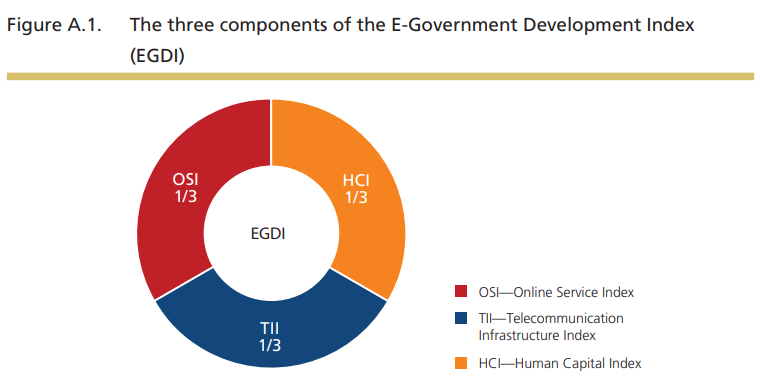
\includegraphics[width=1\linewidth]{figuras/egdi_componentes.png}
    \label{fig:egdi_componentes}
    \footnotesize{Fonte: \cite{ONU_EGDI_description}.}
\end{figure}

De maneira detalhada, a tabela \ref{tab:egdi_componentes_subindices} mostra os sub-índices do EGDI.

\begin{table}[H]
	\centering
	\caption{EGDI: componentes e sub-índices}
	\label{tab:egdi_componentes_subindices}
	\begin{tabular}{|p{5.5cm}|l|}
		\hline
		\textbf{Componentes} & \textbf{Sub-índices} \\
		\hline
		Online Services Index (OSI) & \\
		& Institutional framework (IF) \\ 
		& Services provision (SP) \\
		& Content provision (CP) \\
		& Technology (TEC) \\
		& E-participation (EPI) \\
		\hline
		Telecommunications Infrastructure Index (TII) & Internet users \\
		& Mobile cellular subscribers \\
		& Wireless broadband subscribers \\
		& Broadband affordability \\
		\hline
		Human Capital Index (HCI) & Adult literacy rate (AL) \\
		& Gross enrolment ratio (GER) \\
		& Expected years of schooling (EYS) \\
		& Mean years of schooling (MYS) \\
		& E-government literacy (EGL) \\
		\hline
	\end{tabular}
	\\ \footnotesize{Fonte: elaboração própria baseada em \cite{onu_egov_survey_2024}.}
\end{table}

\cite{ONU_EGDI_EPI_description} conceitua EPI como um índice suplementar derivado do EGDI. O índice de um país reflete os mecanismos de participação cidadã eletrônica que são empregados pelo poder público em comparação a todos os países.

Além disso, \cite{ONU_EGDI_EPI_description} argumenta que o propósito de medição do EPI não é prescrever nenhuma prática específica, mas sim oferecer entendimento de como os países estão usando ferramentas digitais para promover a interação entre o poder público e os cidadãos, e ainda entre o povo, para benefício coletivo.

Os sub-índices do EPI tem como objetivo, conforme \cite{ONU_EGDI_EPI_description} na tabela \ref{tab:epi_subindices}.

\begin{longtable}[c]{@{}ll@{}}
	\caption{Descrição dos sub-índices do EPI}
	\label{tab:epi_subindices}\\
	\toprule
	\textbf{Sub-índice} & \textbf{Descrição}                                                                                  \\* \midrule
	\endfirsthead
	%
	\endhead
	%
	E-information & \begin{tabular}[c]{@{}l@{}}Permitir a participação, fornecendo aos \\ cidadãos informações públicas e acesso à \\ informação sem ou mediante solicitação.\end{tabular}
	\\ \midrule
	E-consultation & \begin{tabular}[c]{@{}l@{}}Engajar os cidadãos em contribuição e \\ deliberações sobre em políticas públicas \\ e os serviços públicos.\end{tabular} 
	\\ \midrule
	E-decision-making & \begin{tabular}[c]{@{}l@{}}Empoderar os cidadãos via co-participação \\ das políticas públicas e co-produção dos \\ componentes dos serviços e as modalidades \\ de entrega.\end{tabular}
	\\ \bottomrule
	\footnotesize{Fonte: elaboração própria baseada em \cite{ONU_EGDI_EPI_description}.}
\end{longtable}

Como exemplo de componente do EGDI, exemplifica-se o OSI. Para \cite{onu_egov_survey_2024}, os valores do OSI, assim como os do EGDI, 

\noindent
\begin{flushleft}
	\setlength{\leftskip}{4cm}
	\small
	"[...]não são medidas absolutas; em vez disso, eles capturam o desempenho digitais dos países de forma relativa uns aos outros em um dado momento. Em razão do OSI é um valor composto, um valor alto é um indicativo de boas práticas em substituição à perfeição. Similarmente, um valor baixo ou que está estagnado desde a edição prévia do relatório da pesquisa\footnote{E-Government Survey da ONU. A relatório da pesquisa foi em 2024 e por ser acessado em \url{https://www.un-ilibrary.org/content/books/9789211067286/read}. A metodologia de cálculo do EGDI é acessível em \url{https://publicadministration.un.org/egovkb/Portals/egovkb/Documents/un/2016-Survey/Annexes.pdf}.}, não significa ausência de progresso no desenvolvimento do governo eletrônico." \cite{onu_egov_survey_2024}
\end{flushleft}

Nota-se como os valores resultados do EGDI não são tratados como medidas absolutas, mas como indicativos da situação do governo eletrônico do país analisado. Como indicador, o EGDI tem grande importância, pois ele vem de um organismo internacional que não tem poder de interferência nos seus Estados-Membros, diferente da União Europeia, por exemplo.

\subsection{EGDI no Brasil e no mundo}

Considerando as informações anteriores, as figuras \ref{fig:mapa_coropletico_paises_egdi}, \ref{fig:mapa_coropletico_paises_epi}, \ref{fig:mapa_coropletico_paises_hci}, \ref{fig:mapa_coropletico_paises_osi} e \ref{fig:mapa_coropletico_paises_tii} contêm mapas coropléticos que mostram o EGDI, seus componentes e o EPI pelo mundo.

\begin{figure}[H]
	\centering
	\caption{EGDI dos países do mundo em 2024}
	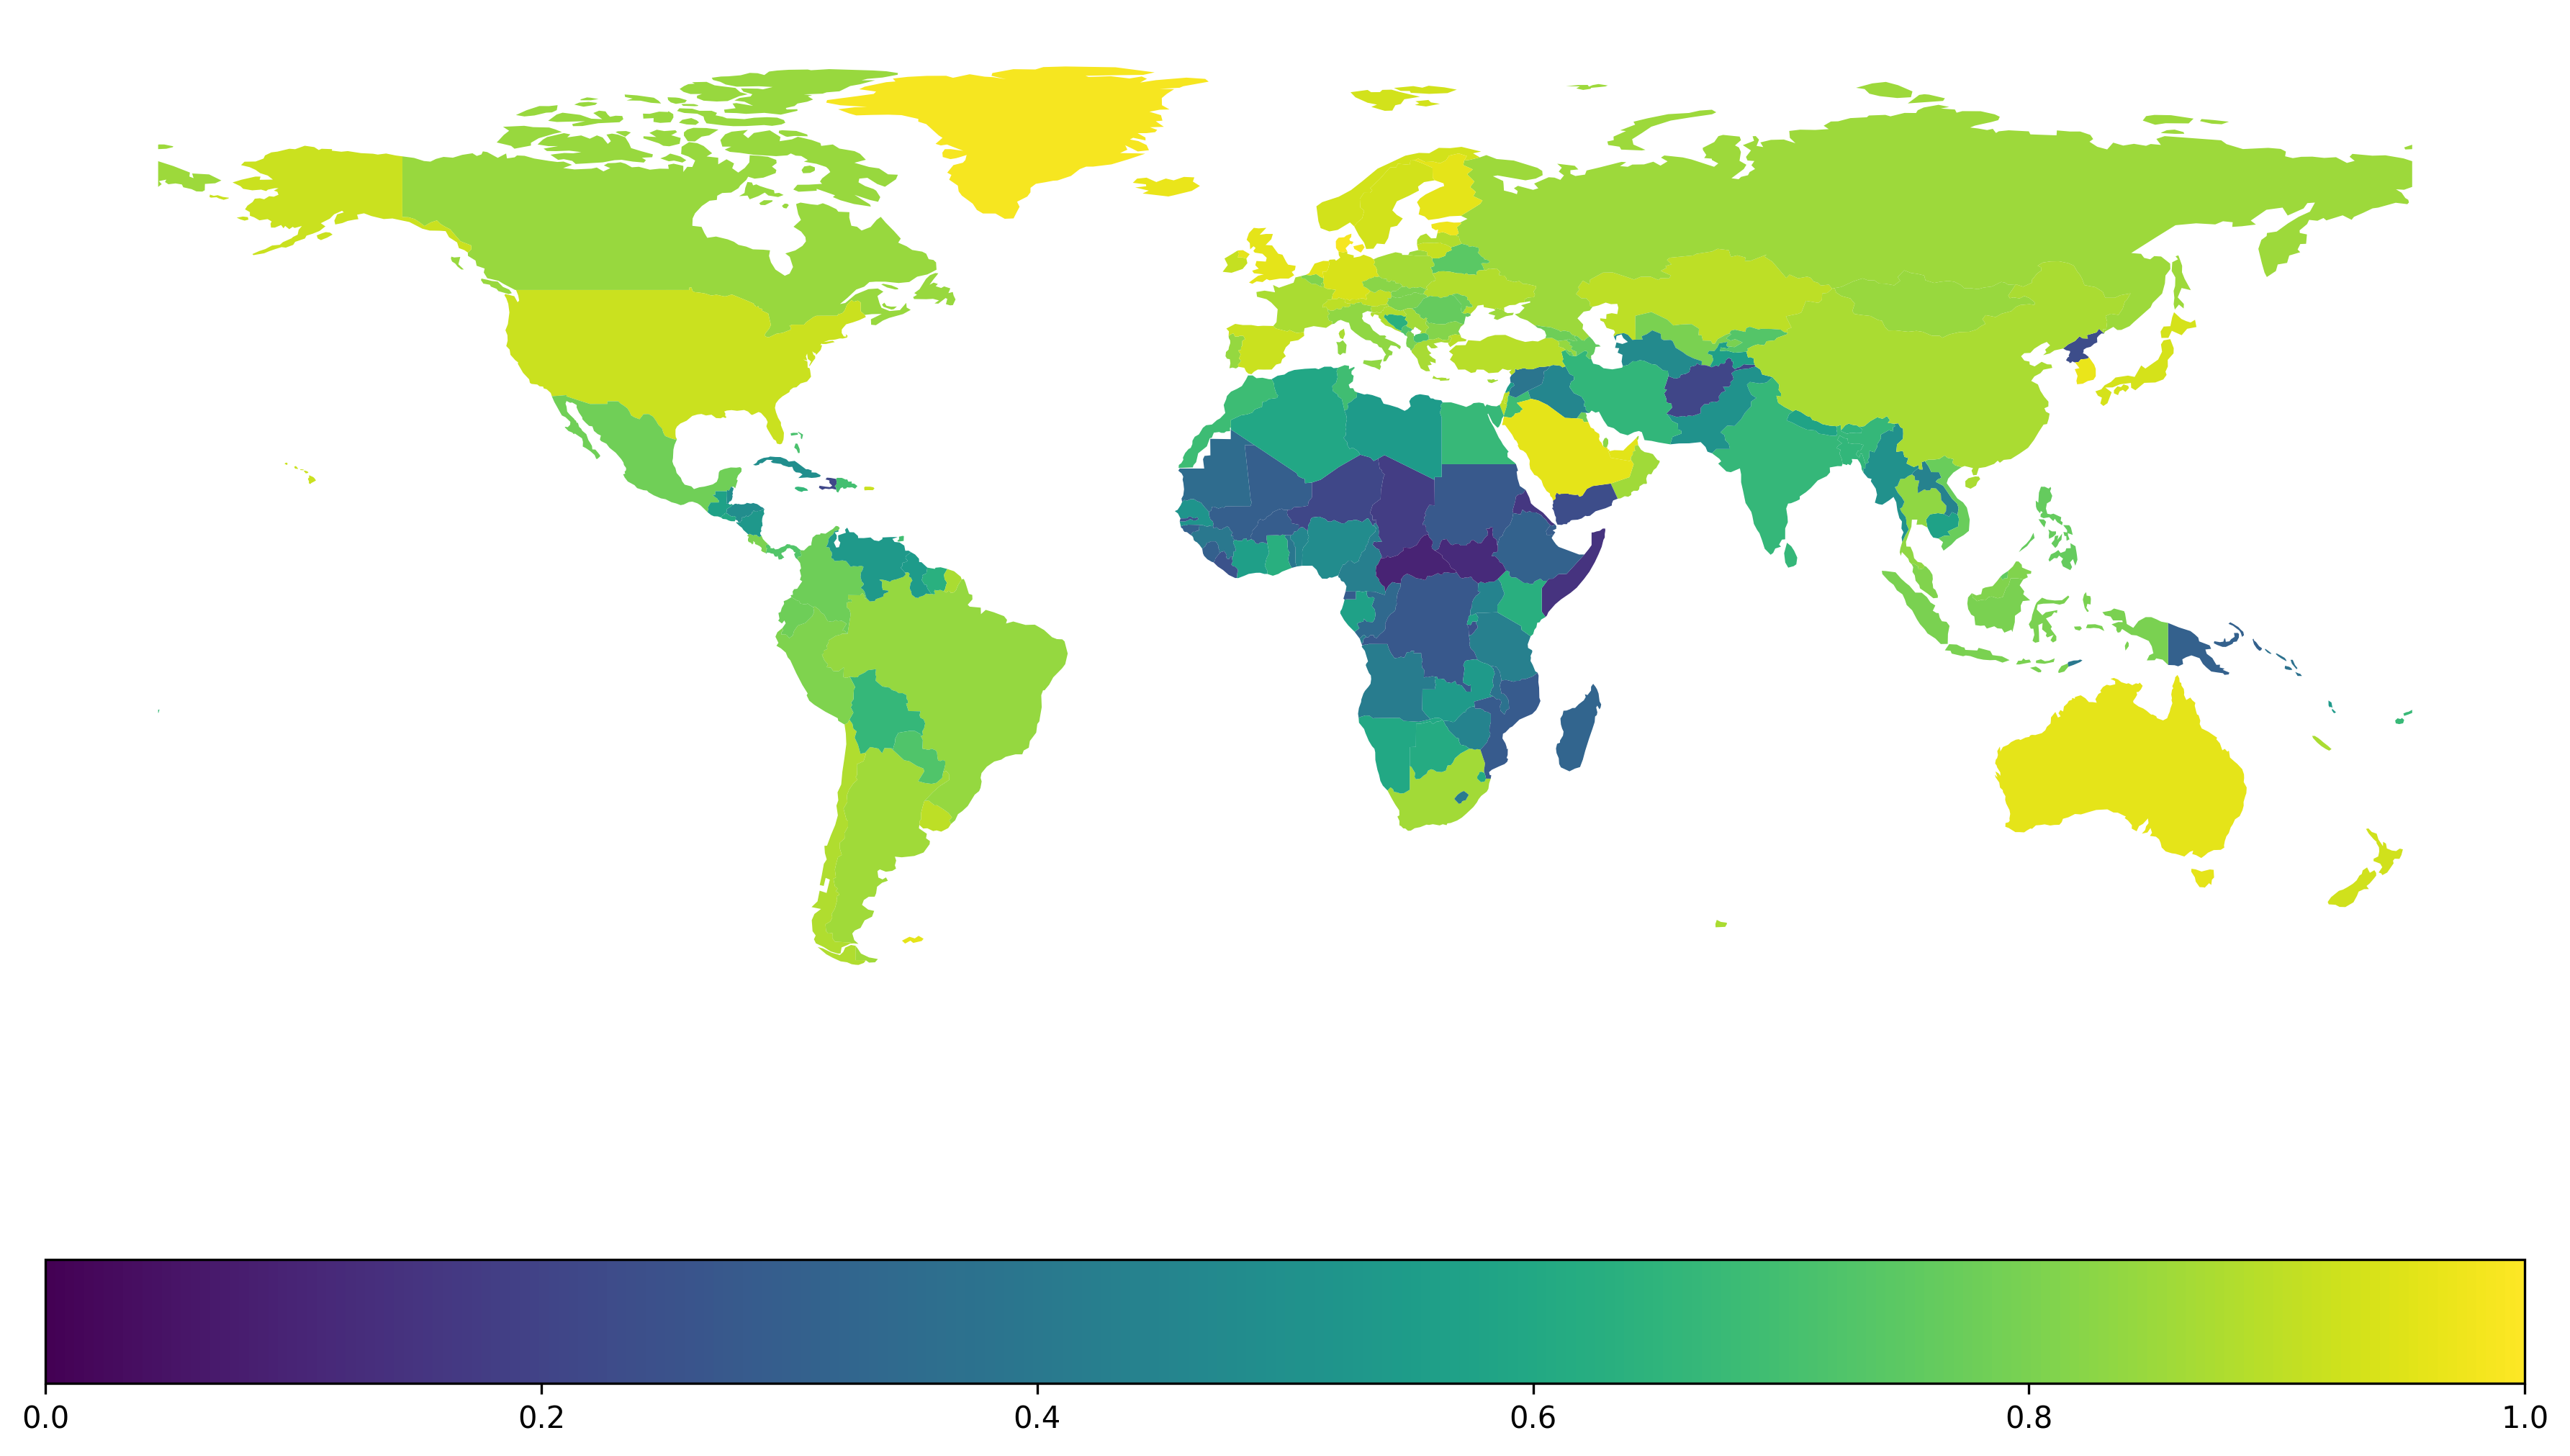
\includegraphics[width=1\linewidth]{figuras/mapa_coropletico_paises_egdi}
	\label{fig:mapa_coropletico_paises_egdi}
	\footnotesize{Fonte: elaboração própria baseada em \cite{ONU_EGDI_dados}.}
\end{figure}

\begin{figure}[H]
	\centering
	\caption{EPI dos países do mundo em 2024}
	
\includegraphics[width=1\linewidth]{figuras/mapa_coropletico_paises_epi}
	\label{fig:mapa_coropletico_paises_epi}
	\footnotesize{Fonte: elaboração própria baseada em \cite{ONU_EGDI_dados}.}
\end{figure}

\begin{figure}[H]
	\centering
	\caption{HCI dos países do mundo em 2024}
	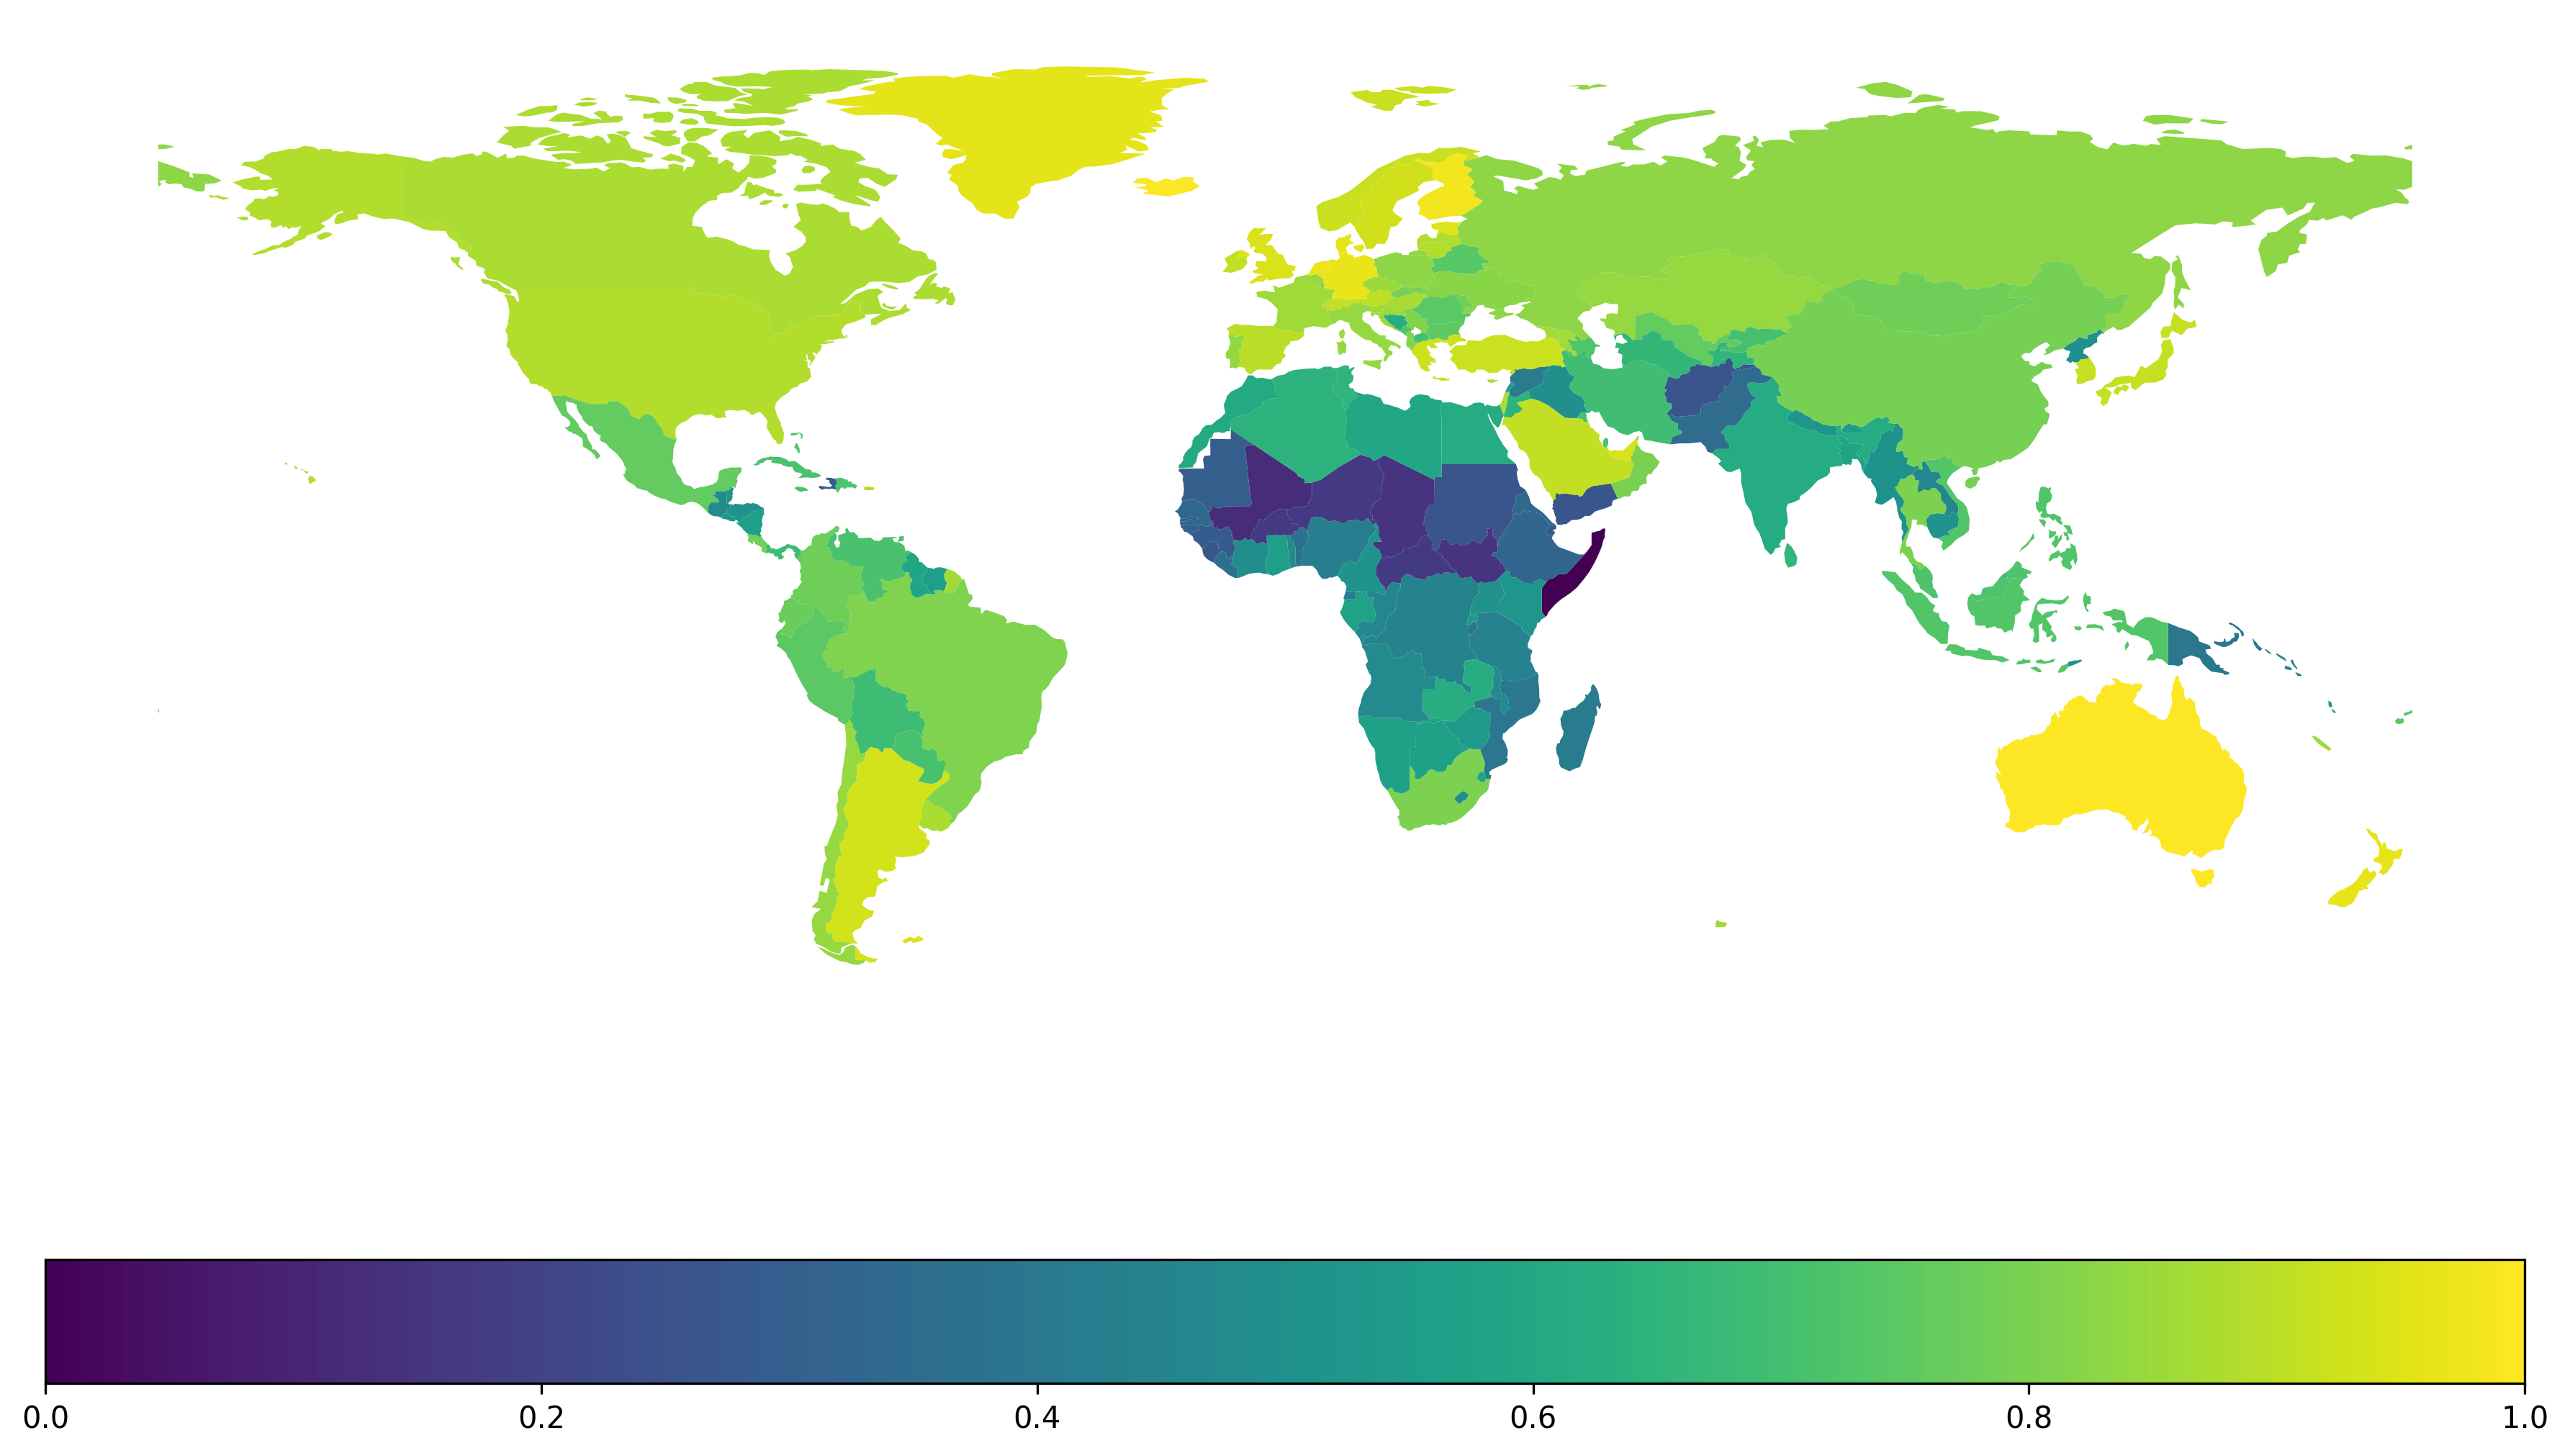
\includegraphics[width=1\linewidth]{figuras/mapa_coropletico_paises_hci}
	\label{fig:mapa_coropletico_paises_hci}
	\footnotesize{Fonte: elaboração própria baseada em \cite{ONU_EGDI_dados}.}
\end{figure}

\begin{figure}[H]
	\centering
	\caption{OSI dos países do mundo em 2024}
	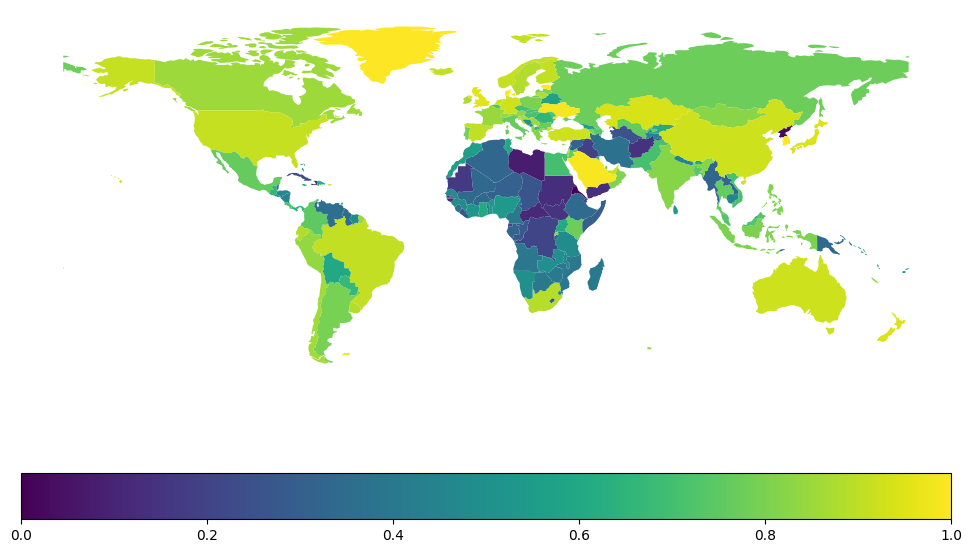
\includegraphics[width=1\linewidth]{figuras/mapa_coropletico_paises_osi}
	\label{fig:mapa_coropletico_paises_osi}
	\footnotesize{Fonte: elaboração própria baseada em \cite{ONU_EGDI_dados}.}
\end{figure}

\begin{figure}[H]
	\centering
	\caption{TII dos países do mundo em 2024}
	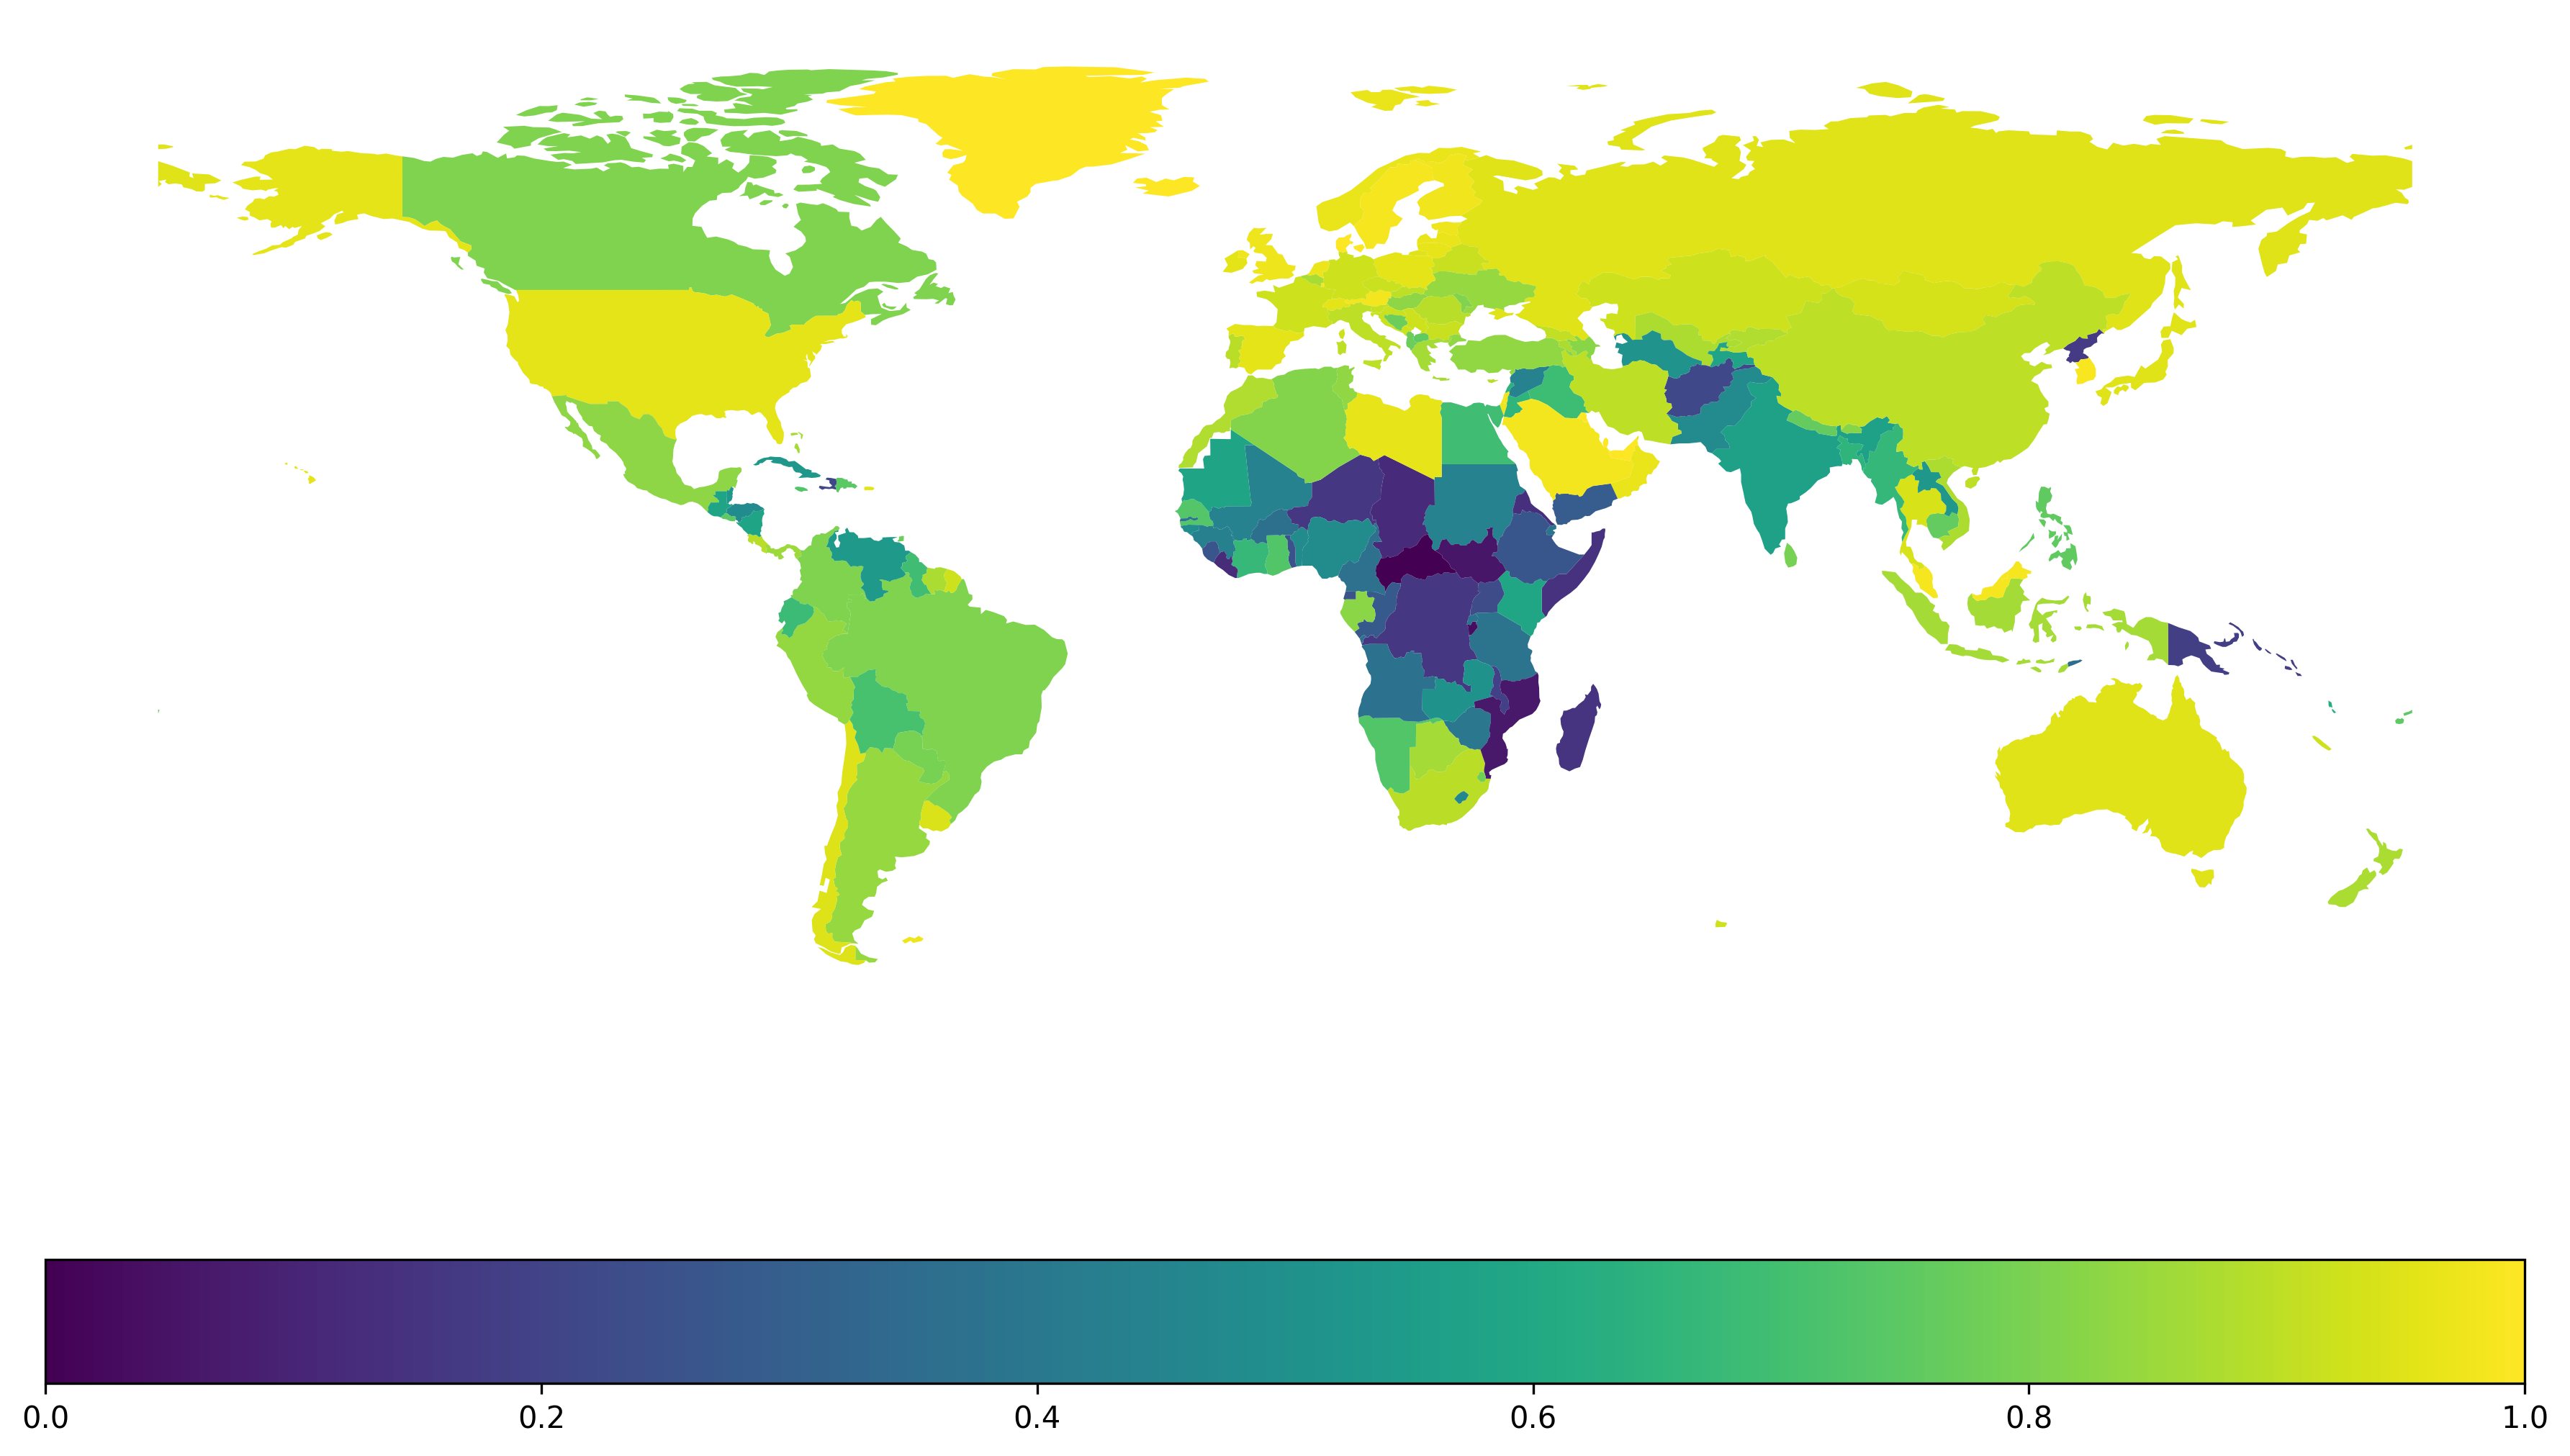
\includegraphics[width=1\linewidth]{figuras/mapa_coropletico_paises_tii}
	\label{fig:mapa_coropletico_paises_tii}
	\footnotesize{Fonte: elaboração própria baseada em \cite{ONU_EGDI_dados}.}
\end{figure}

Conforme exposto pelas figuras \ref{fig:mapa_coropletico_paises_egdi}, \ref{fig:mapa_coropletico_paises_epi}, \ref{fig:mapa_coropletico_paises_hci}, \ref{fig:mapa_coropletico_paises_osi} e \ref{fig:mapa_coropletico_paises_tii}, o Brasil se destaca sempre tendo pontuação em alta em qualquer indicador. Para entender a situação do Brasil, comparou-se seu EGDI, seus componentes e o EPI com a média mundial. A figura \ref{fig:comparacao_egdi_brasil_mundo} expõe os valores do EGDI, seus componentes e o EPI do Brasil e a média mundial.

\begin{figure}[H]
	\centering
	\caption{EGDI, seus sub-índices e o EPI do Brasil e a média mundial em 2024}
	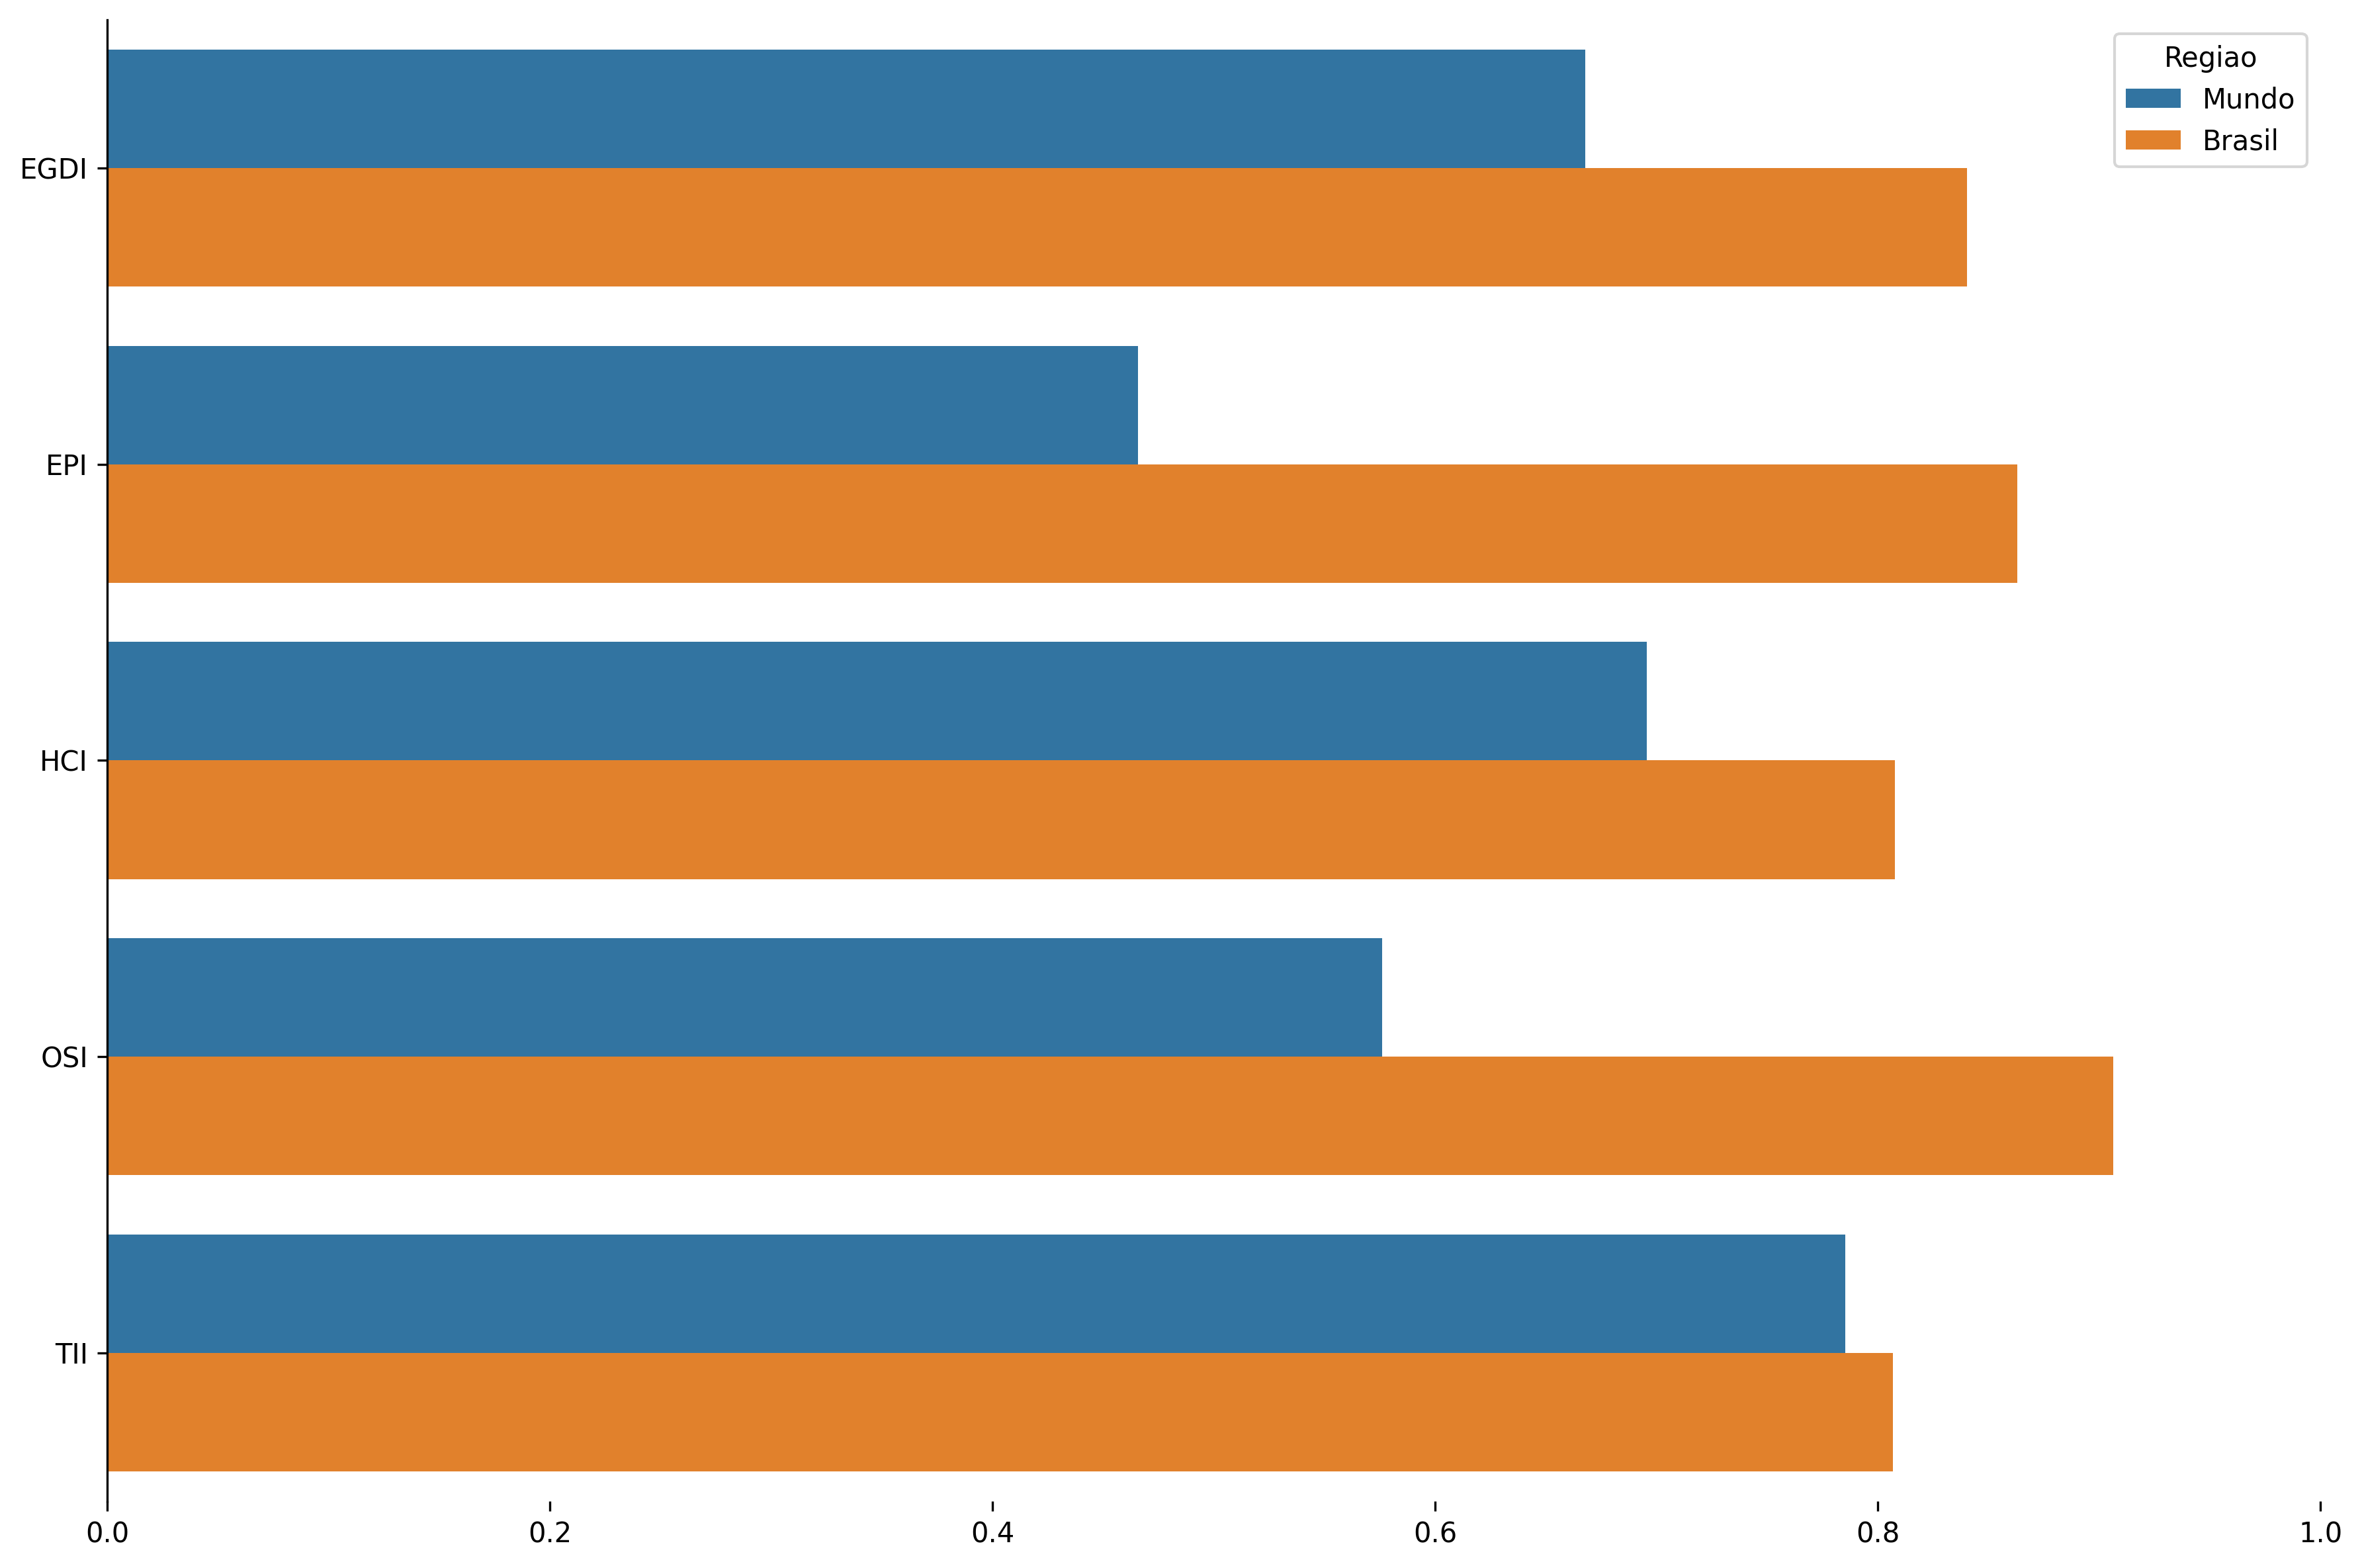
\includegraphics[width=1\linewidth]{figuras/comparacao_egdi_brasil_mundo}
	\label{fig:comparacao_egdi_brasil_mundo}
	\footnotesize{Fonte: elaboração própria baseada em \cite{ONU_EGDI_dados}.}
\end{figure}

Da análise da figura \ref{fig:comparacao_egdi_brasil_mundo}, destaque que o Brasil está acima da média mundial em todos os indicadores. Apenas o TII mundial se aproxima do valor atingido pelo Brasil. Concomitantemente, analisou-se se o EGDI tem relação com o índice de democracia, PIB \textit{per capita} PPC em dólares dos Estados Unidos e com os gastos públicos como porcentagem do PIB eleitoral.

Quando o EGDI foi comparado com o índice de democracia eleitoral, descobriu-se que o coeficiente de correlação é 0,2975. Em razão da fraca correlação entre EGDI e índice de democracia eleitoral, optou-se pelo PIB \textit{per capita} PPC em dólares dos Estados Unidos e pelos gastos públicos como porcentagem do PIB. Assim, objetivando descobrir se há correlação entre o PIB \textit{per capita} PPC em dólares dos Estados Unidos e gastos públicos como porcentagem do PIB com o EGDI, seus componentes e o EPI, foram descobertos e analisados os coeficientes de correlação resultantes dos relacionamentos citados.

O resultado foi dividido nas figuras \ref{fig:correlacao_egdi_indicedemocraciaeleitoral}, \ref{fig:correlacao_egdi_pibpercapitapcc} e \ref{fig:correlacao_egdi_gastospublicos}.

\begin{figure}[H]
	\centering
	\caption{Coeficientes de correlação entre EGDI, seus componentes e o EPI com o índice de democracia eleitoral}
	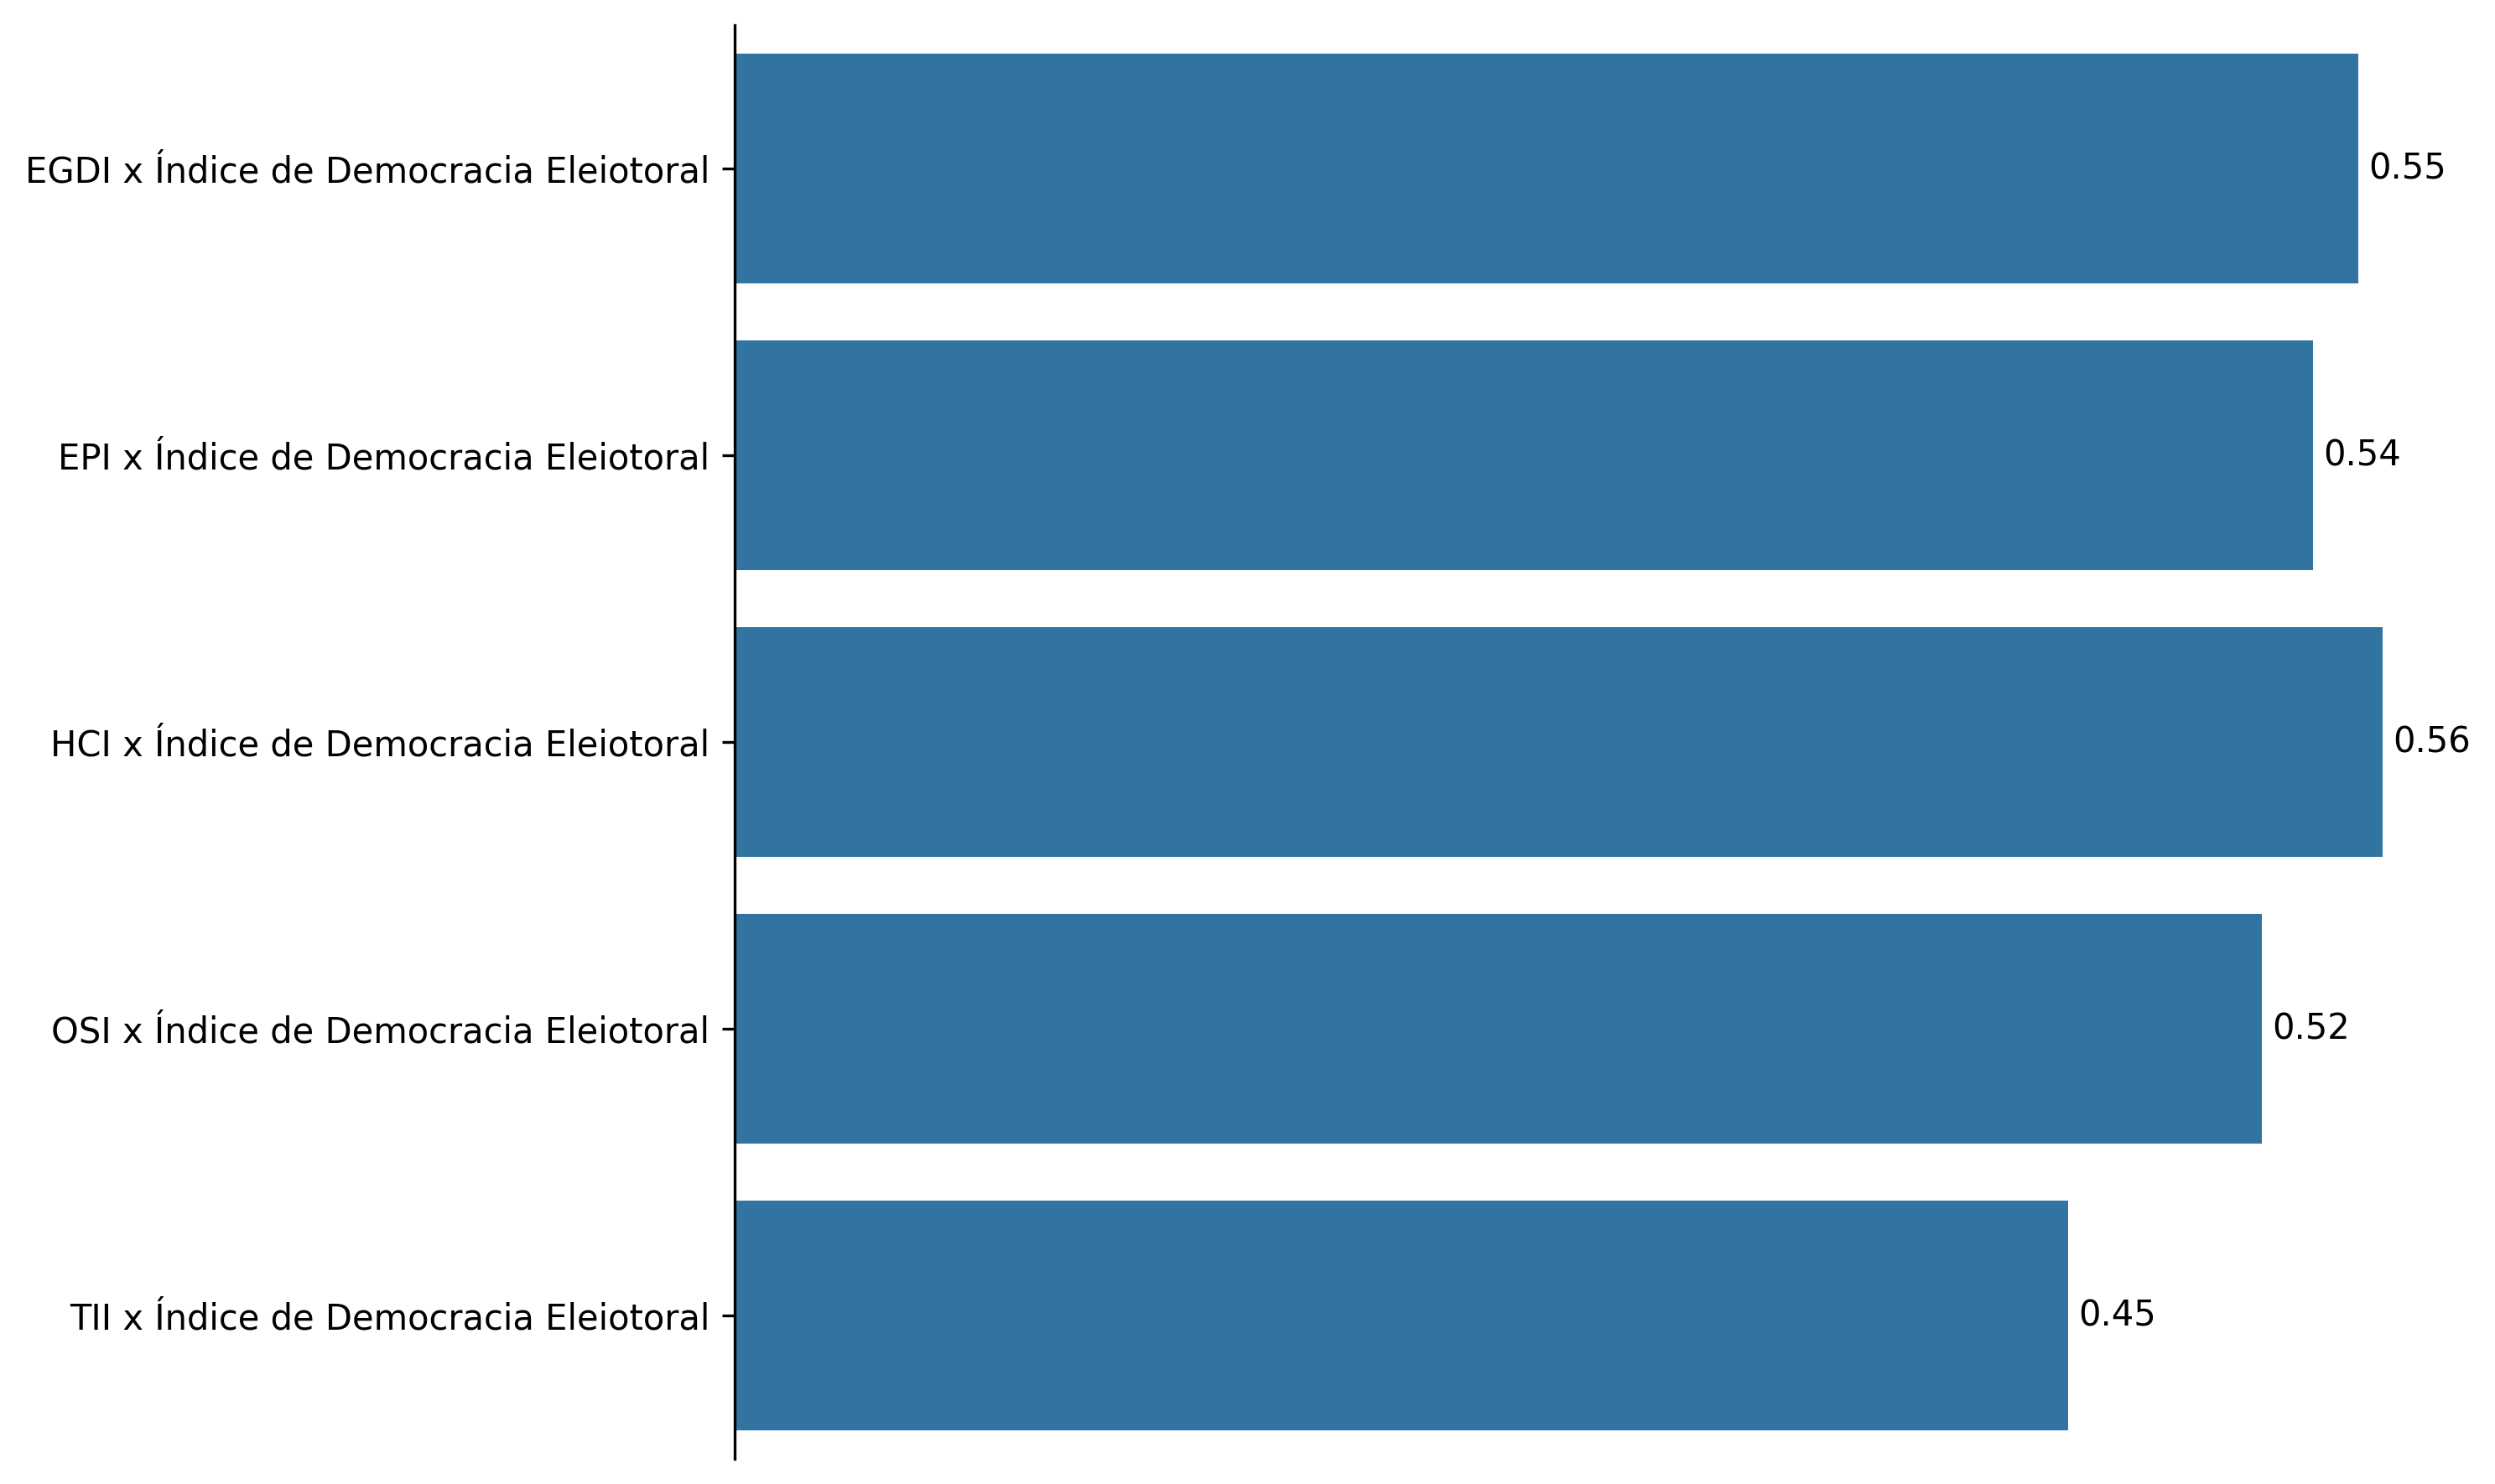
\includegraphics[width=1\linewidth]{figuras/correlacao_egdi_indicedemocraciaeleitoral.png}
	\label{fig:correlacao_egdi_indicedemocraciaeleitoral}
	\footnotesize{Fonte: elaboração própria baseada em \cite{electoral-democracy-index} e \cite{ONU_EGDI_dados}.}
\end{figure}

\begin{figure}[H]
	\centering
	\caption{Coeficientes de correlação entre EGDI, seus componentes e o EPI com o PIB \textit{per capita} PPC}
	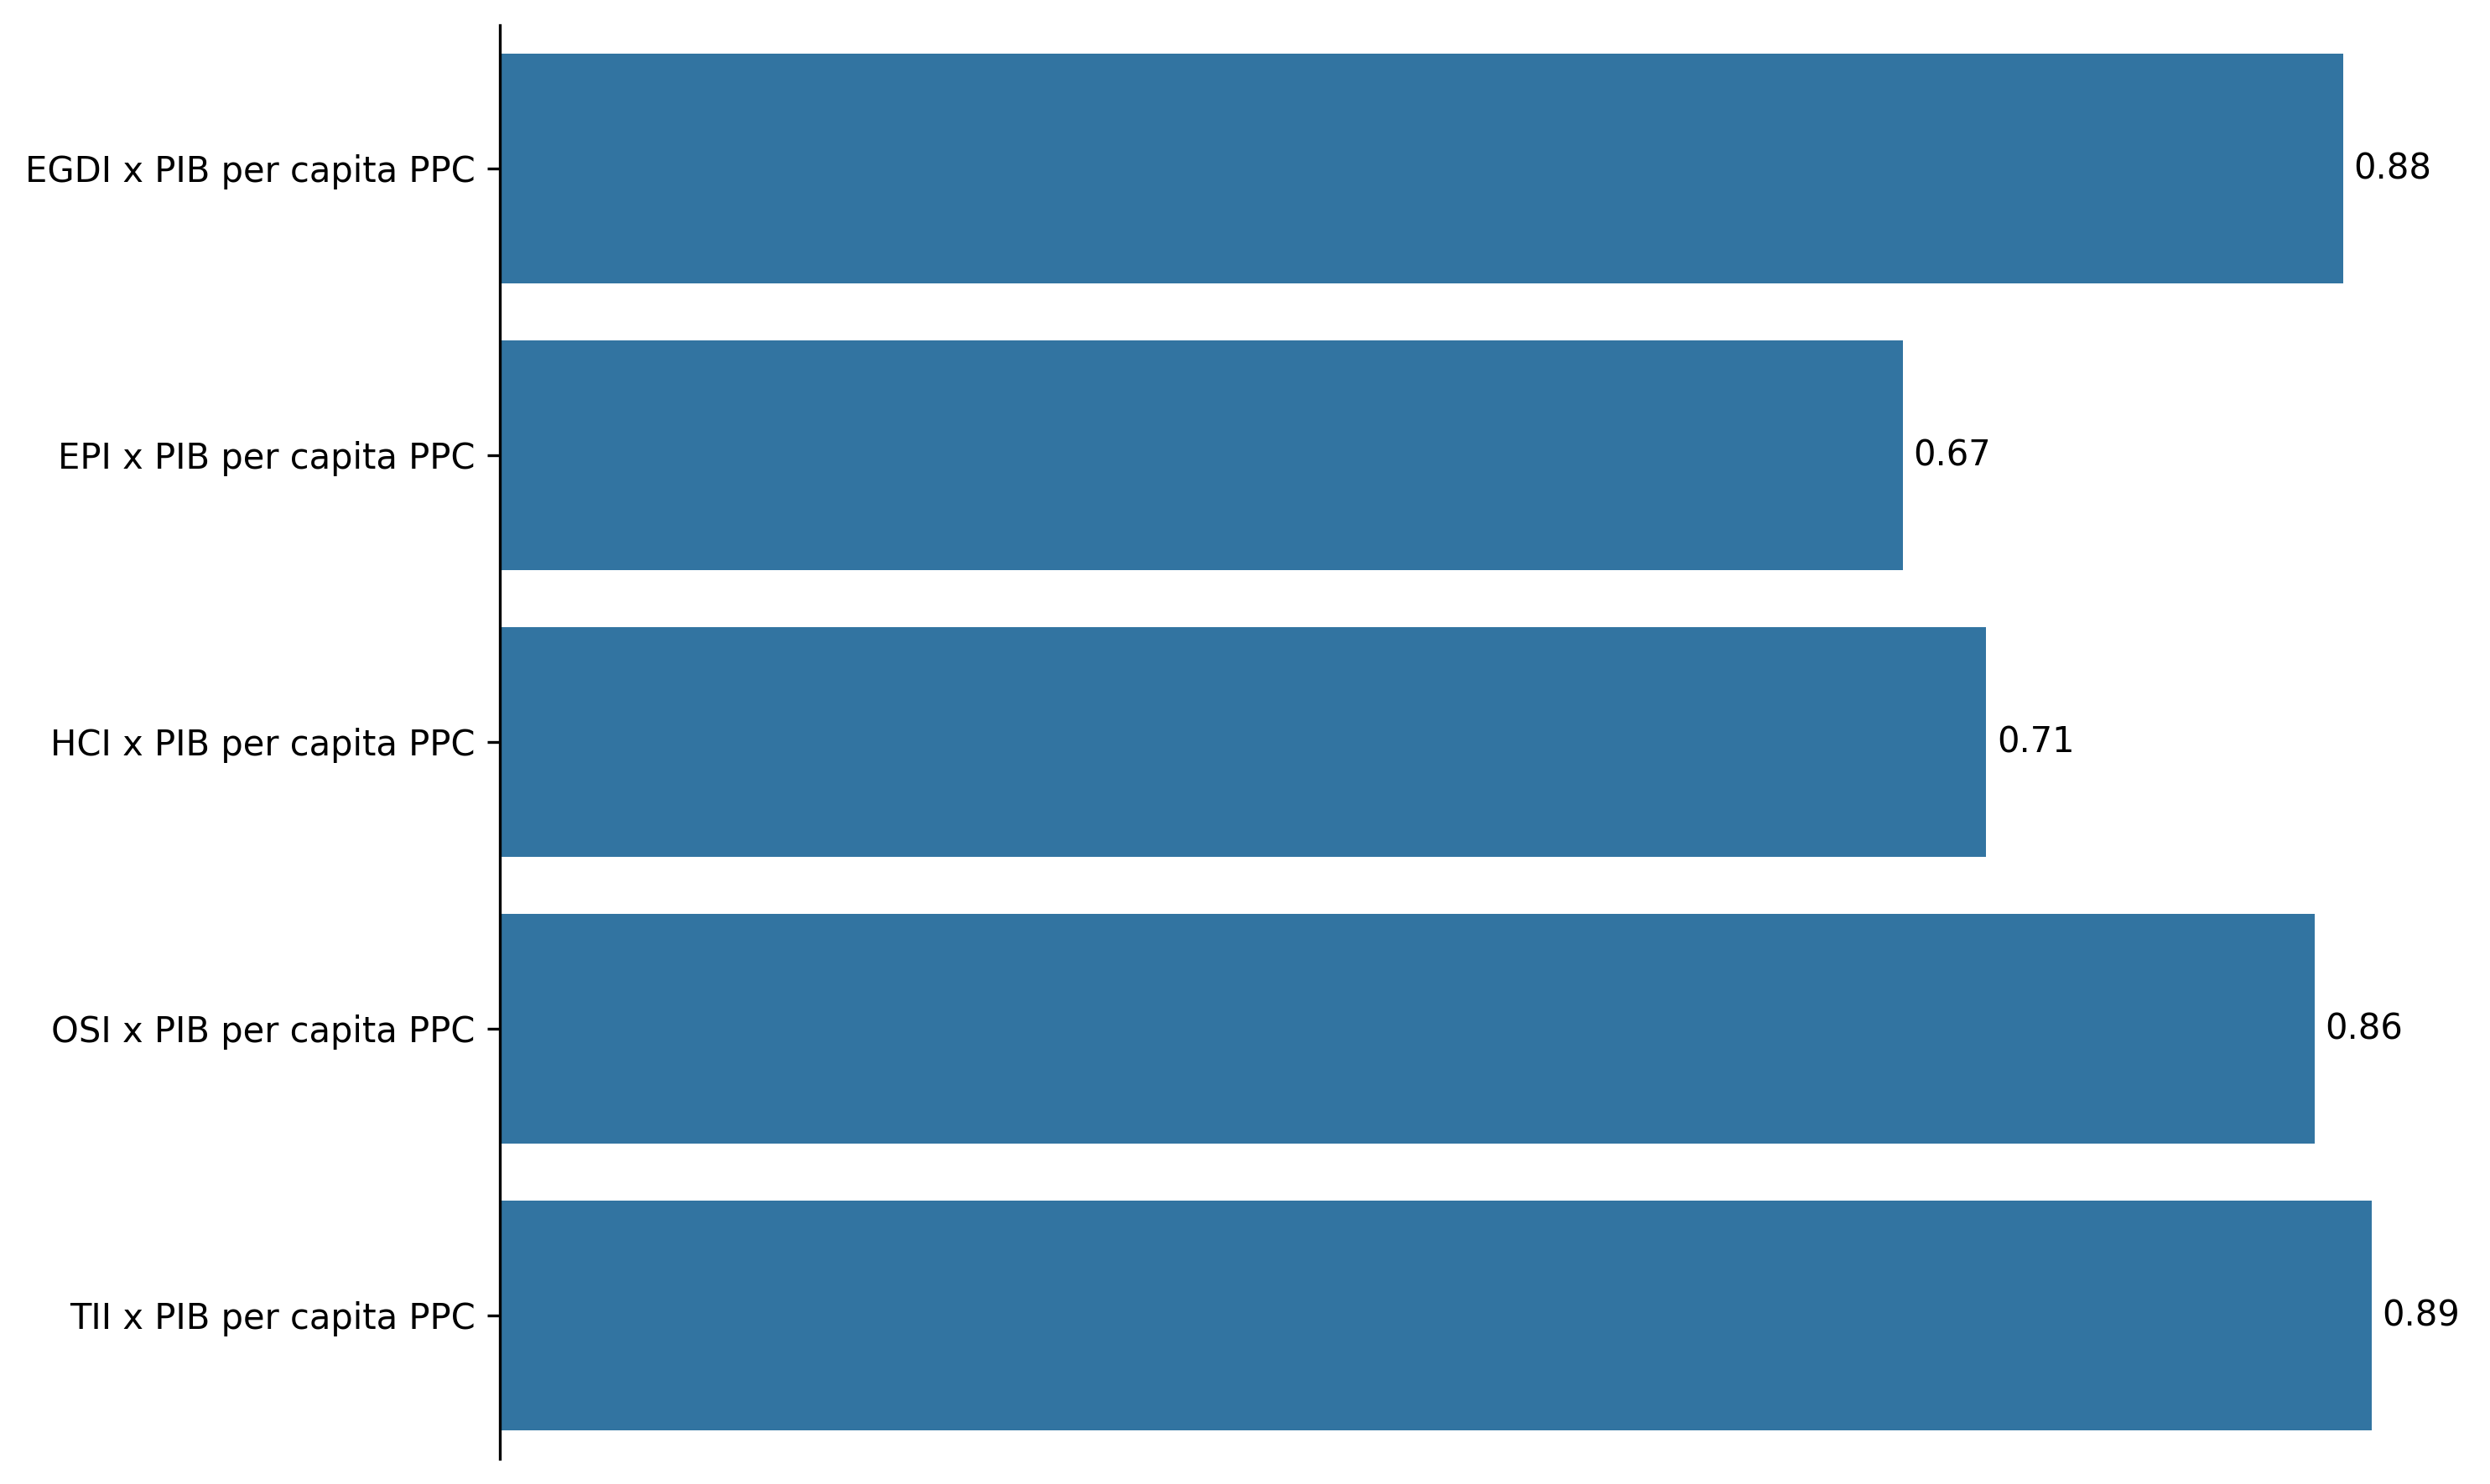
\includegraphics[width=1\linewidth]{figuras/correlacao_egdi_pibpercapitapcc.png}
	\label{fig:correlacao_egdi_pibpercapitapcc}
	\footnotesize{Fonte: elaboração própria baseada em \cite{WB_pib_per_capita_países}.}
\end{figure}

\begin{figure}[H]
	\centering
	\caption{Coeficientes de correlação entre EGDI, seus componentes e o EPI com os gastos públicos como percentual do PIB}
    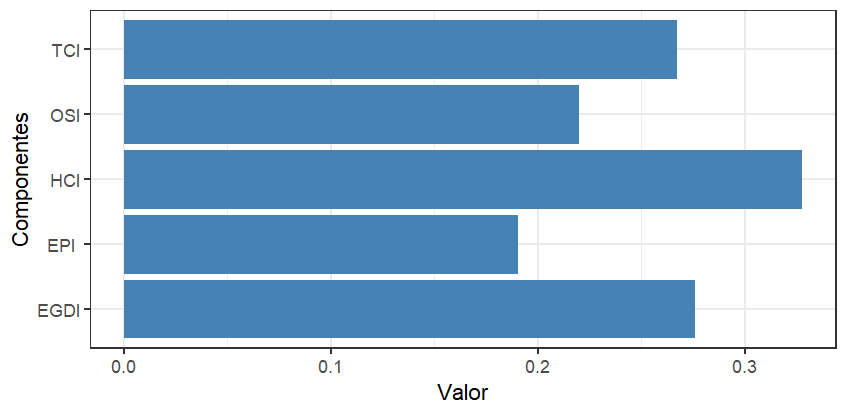
\includegraphics[width=1\linewidth]{figuras/correlacao_egdi_gastospublicos.png}
	\label{fig:correlacao_egdi_gastospublicos}
	\footnotesize{Fonte: elaboração própria baseada em \cite{FMI_gov_expenditure}.}
\end{figure}

Descobriu-se que o EGDI, seus componentes e o EPI quando comparados com o PIB \textit{per capita} PPC têm coeficientes de correlação acima de 0,6, o que indica que há correlação forte entre as variáveis. Do resultado, deduz-se que há uma tendência do crescimento do PIB de afetar positivamente o EGDI, que seguiria a tendência de crescimento.

Já a relação entre o EGDI, seus componentes e o EPI quando comparados com os gastos públicos como percentual do PIB indica uma fraca correlação, que, no máximo, passou um pouco de 0,3. Disso, extrai-se o entendimento de que as variáveis são independentes entre si.

Resumidamente, interpreta-se que quanto mais economicamente forte for um país, mais orçamento público ele tem disponível para investir em digitalização do serviço público. Contrariamente, gastos públicos como percentual do PIB não interferem no aspecto do governo eletrônico, pois demonstram que há múltiplos objetivos do poder público a serem executados na forma de gastos públicos, não exclusivamente ligados a governo eletrônico.

\cite{singh2007country}, em seu artigo de 2007, cita que uma explicação possível para o padrão de resultados observados - a baixa correlação entre a importância das tecnologias de informação e comunicação com a governança pública - indica que as novidades apresentadas pelas TIC limitam o governo eletrônico.

Complementarmente, \cite{singh2007country} argumenta que, como novas tecnologias inovadoras têm custo financeiro e conferem benefícios aos que podem ter acesso a elas. Contudo, à medida que são utilizadas para implementar governo eletrônico, se tornam mais acessíveis. Como consequência, o papel mediador principal da infraestrutura de TIC pode ser enfraquecido; enquanto o capital humano e a qualidade da governança podem ganhar influência.

 Considerando o argumento de \cite{singh2007country}, ele reforça a importância de indicadores como o EGDI para a implementação de governo eletrônico, pois à medida os custos de criação e implementação de novas tecnologias são democratizados, é possível expandir a infraestrutura de TIC do governo eletrônico para focar na melhora dos demais componentes do EGDI.

Além da ideia supracitada, \cite{singh2007country} reforça a noção de que altos gastos públicos como porcentagem do PIB não impactam em um valor equivalente de EGDI.

\subsection{Revisão da literatura}

Corroborando a análise desta seção, apresentar-se-ão ideias de diversos autores via revisão da literatura.

Inicialmente, \cite{alisherovna2021whether} chegou a uma conclusão similar presente nesta seção, demonstrando que o EGDI impacta positivamente a taxa de crescimento do PIB dos países, conforme demonstrado na figura \ref{fig:usmanova_egdi_gdp}.

\begin{figure}[H]
	\centering
	\caption{Como os países são posicionados em torno do EGDI de acordo com sua taxa de crescimento do PIB}
	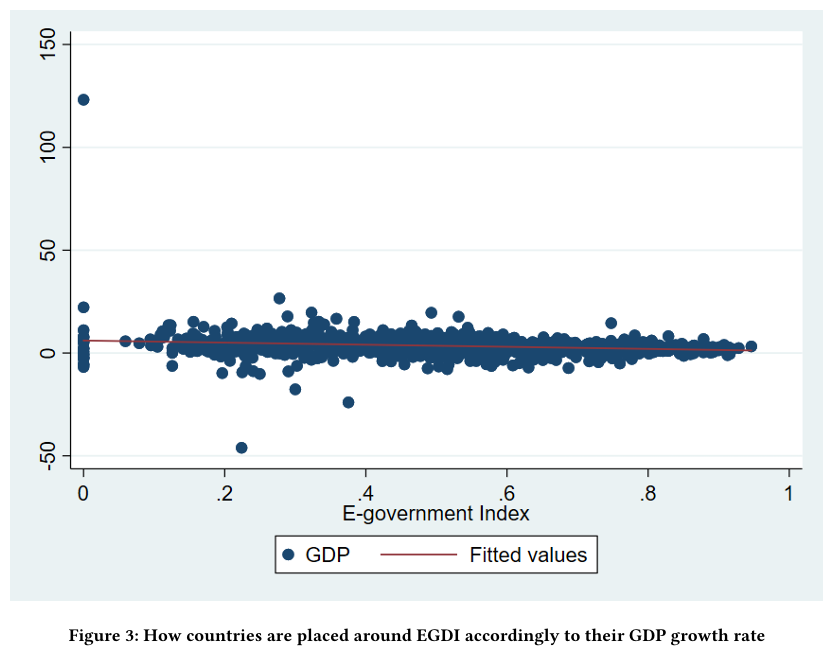
\includegraphics[width=1\linewidth]{figuras/usmanova_egdi_gdp}
	\label{fig:usmanova_egdi_gdp}
	\footnotesize{Fonte: \cite{alisherovna2021whether}.}
\end{figure}

Da figura \ref{fig:usmanova_egdi_gdp}, nota-se como os pontos estão muito próximos da linha de tendência, o que indica forte correlação. Tal como a forte apresentada na figuras \ref{fig:correlacao_egdi_pibpercapitapcc}, o EGDI tem influência em vários aspectos do PIB.

\cite{scatterplot_egdi_2024} encontrou uma conclusão diferente de \cite{alisherovna2021whether}, conforme exposto na figura \ref{fig:UN_EGDI_EGDI_scatter}.

\begin{figure}[H]
	\centering
	\caption{Gráfico de dispersão do EGDI de 2024}
	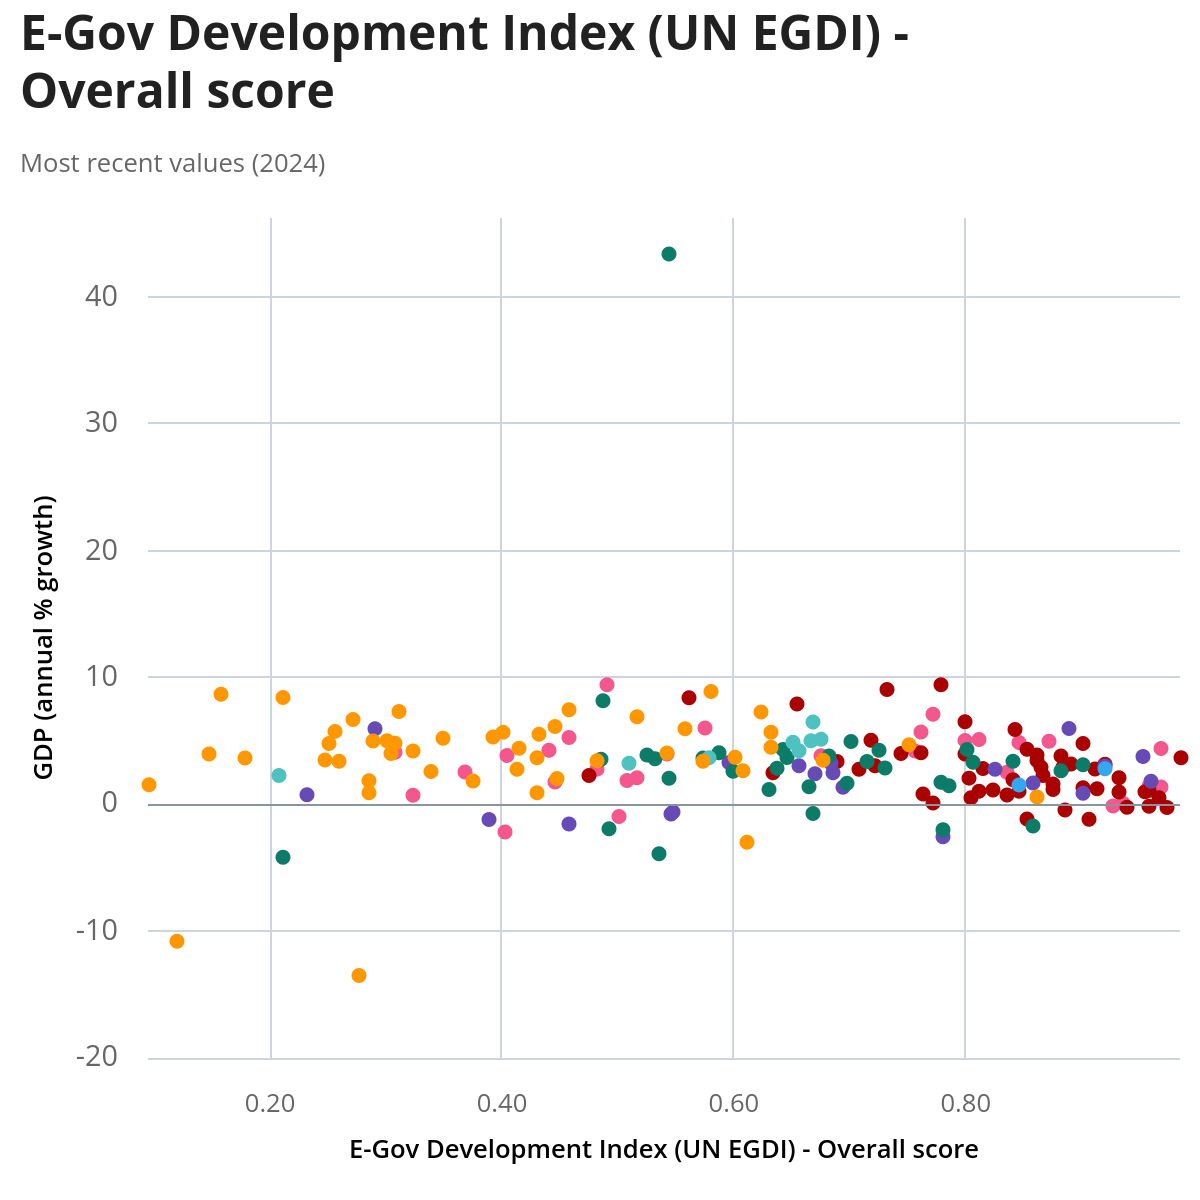
\includegraphics[width=1\linewidth]{figuras/UN_EGDI_EGDI_scatter}
	\label{fig:UN_EGDI_EGDI_scatter}
	\footnotesize{Fonte: \cite{scatterplot_egdi_2024}.}
\end{figure}

Nota-se a diferença entre as figuras \ref{fig:usmanova_egdi_gdp} e \ref{fig:UN_EGDI_EGDI_scatter}, de 2021 e 2024, respectivamente. A figura \ref{fig:UN_EGDI_EGDI_scatter} mostra a correlação fraca ou mesmo a ausência de correlação entre EGDI e taxa anual de crescimento do PIB. A diferença temporal de 4 anos pode ser a justificativa para os resultados divergentes. Outra diferença notável é que o pontos do EGDI da figura \ref{fig:UN_EGDI_EGDI_scatter} estão mais concentrados quando o EGDI é mais alto.

Em segundo lugar, \cite{kotenok2020government} argumenta que em sua pesquisa, partiu-se do princípio de que o governo eletrônico tem um impacto direto ou indireto, ou ambos, na economia; a análise de regressão em painel que utiliza o índice do PIB como variável dependente forneceu uma ideia intuitiva de que o índice desenvolvido tem um impacto potencial nos processos econômicos.

Em razão do pressuposto apresentado no parágrafo anterior, \cite{kotenok2020government} complementa que podem concluir
que o impacto do governo eletrônico pode impulsionar a inovação ou
mesmo ser um componente importante na compreensão de como a
economia é transformada devido à tecnologia.

Em terceiro lugar, \cite{kumar2020cultural} cita que seu estudo utiliza dados secundários sobre cultura nacional e desenvolvimento do governo eletrônico para explorar as relações entre as dimensões culturais e o desenvolvimento do governo eletrônico. Pode-se concluir, a partir deste estudo, que a cultura nacional influencia significativamente o desenvolvimento do governo eletrônico em um país.

\cite{kumar2020cultural} complementa que uma pesquisa das Nações Unidas indica que o desenvolvimento de um programa de governo eletrônico culturalmente relevante aproxima os cidadãos do governo. Os resultados mostraram que o aspecto de que o desenvolvimento econômico, medido pelo PIB per capita, desempenha um papel importante na indicação da preferência por serviços de governo eletrônico.

\cite{kumar2020cultural} finaliza argumentando que cultura e desenvolvimento econômico estão inter-relacionados. Portanto, os países desenvolvidos e em desenvolvimento respondem de forma diferente à recepção do governo eletrônico.

Finalmente, \cite{ziolo2022government} argumenta que a análise fornece diversas conclusões de significativa importância cognitiva e prática, especialmente do ponto de vista da compreensão dos fatores de crescimento e da definição das diretrizes da política econômica. Ao destacar a intensidade dos processos de desenvolvimento da administração eletrônica, os autores apontaram seu impacto nas esferas ambiental, social e econômica, relevantes para o crescimento sustentável.

\cite{ziolo2022government} descobriu que a correlação observada entre o nível de desenvolvimento do governo eletrônico e as áreas ambiental, social e econômica parece ser significativa. Essa correlação implica que a digitalização dos processos administrativos pode ter um impacto real no desenvolvimento sustentável,
promovendo, assim, mudanças positivas em todas as suas três esferas.

Para \cite{ziolo2022government}, o que parece extremamente importante para os processos de tomada de decisão é a relação adicional revelada entre as áreas investigadas acima em relação aos desfasamentos temporais. Em razão disso,  investir no desenvolvimento de infraestrutura digital e serviços eletrônicos governamentais traz múltiplos benefícios reais a longo prazo e tem um impacto direto em todas as três áreas relevantes para o desenvolvimento sustentável moderno.

De forma conclusiva, para \cite{ziolo2022government}, essa relação de longo prazo é particularmente relevante para identificar questões ambientais cujos efeitos parecem se manifestar claramente 10 a 15 anos após a implementação de medidas administrativas. Isso é fortemente evidente no caso da variável que representa a contribuição dos impostos ambientais para o PIB. Essa variável é considerada hoje um indicador da nossa evolução rumo à economia verde.

Adicionalmente, a figura \ref{fig:egdi_brasil_2003_2024} mostra como o EGDI do Brasil mudou desde 2003 até 2024. 

\begin{figure}[H]
	\centering
	\caption{EGDI, seus componentes e do EPI no Brasil (2003-2005, 2008-2024 bienalmente)}
	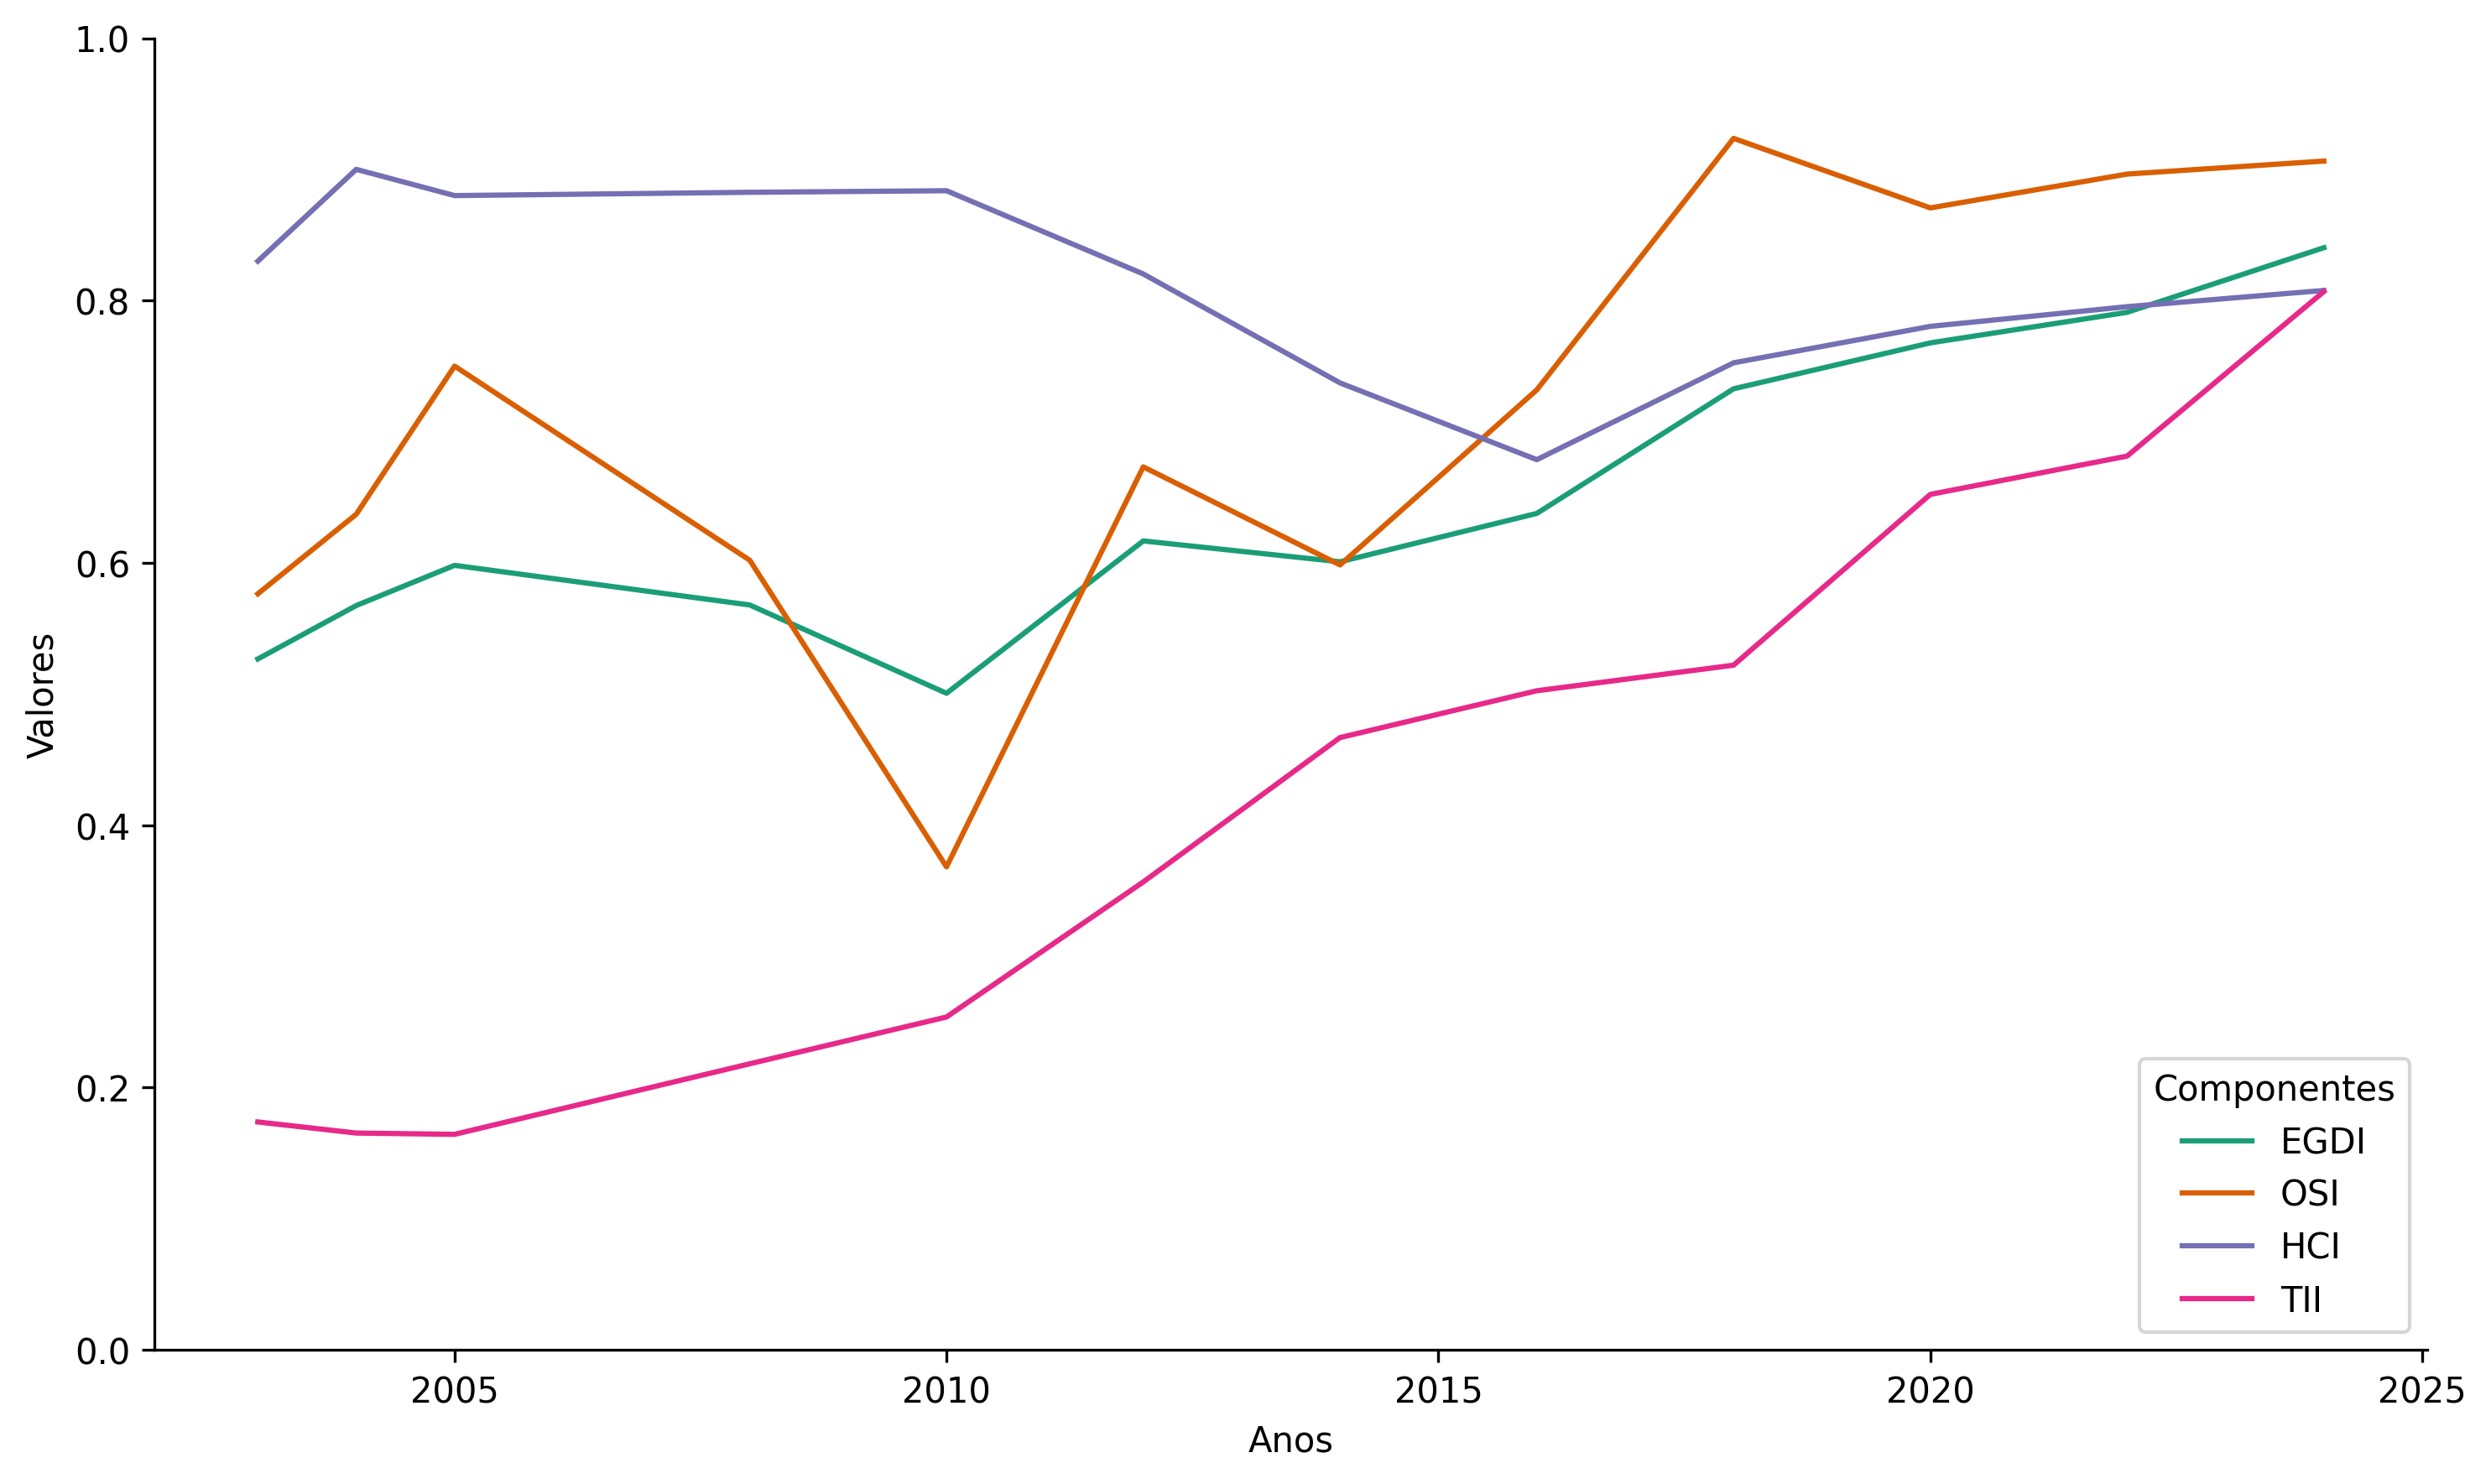
\includegraphics[width=1\linewidth]{figuras/egdi_brasil_2003_2024.PNG}
	\label{fig:egdi_brasil_2003_2024}
	\footnotesize{Fonte: \cite{ONU_EGDI_dados}.}
\end{figure}

Nota-se como o TII foi o componente que mais cresceu de forma contínua; já o OSI teve a maior queda, porém o componente que atingiu o nível mais alto de todos os componentes. O HCI foi o único componente em teve queda no valor. Por fim, o EGDI teve unas quedas, porém voltou a subir.

\subsection{Indicadores de TIC de governo eletrônico}
\label{indicadores_tic_egov}

A ONU tem os indicadores de TIC de governo eletrônico como algo complementar ao EGDI. Os indicadores são, conforme \cite{ONU_ICT_in_government_indicators}:

\begin{itemize}
	\item Existência de estratégia nacional de governo eletrônico ou equivalente;
	\item Existência de identidade digital para acessar ou outra forma de autenticação requerida para poder acessar serviços digitais;
	\item Existência de um portal de compras governamentais.
\end{itemize}

Os resultados globais dos indicadores estão presentes nas figuras \ref{fig:national_government_strategy}, \ref{fig:national_identity} e \ref{fig:procurement_portal}.

\begin{figure}[H]
	\centering
	\caption{Indicador de TIC de governo eletrônico: Existência de estratégia nacional de governo eletrônico ou equivalente}
	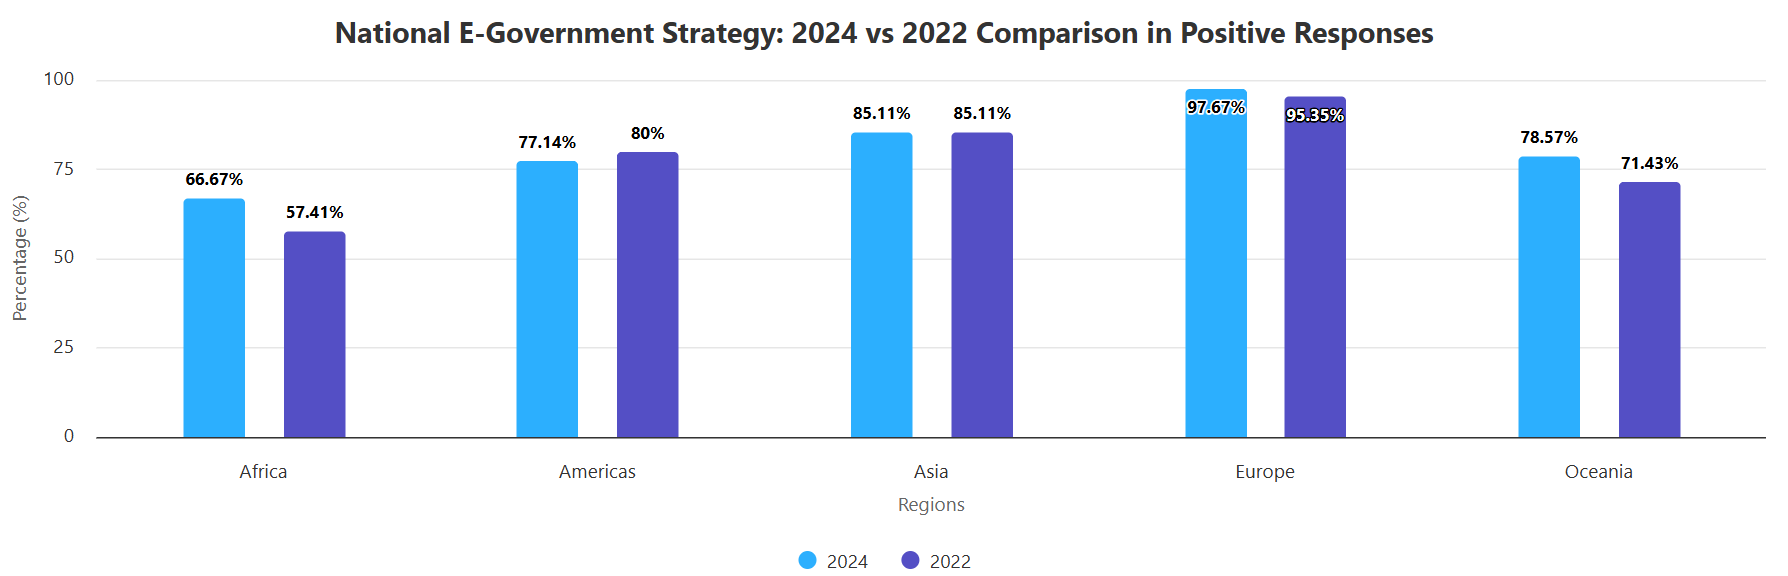
\includegraphics[width=1\linewidth]{figuras/national_government_strategy}
	\label{fig:national_government_strategy}
	\footnotesize{Fonte: \cite{ONU_ICT_in_government_indicators}.}
\end{figure}

\begin{figure}[H]
	\centering
	\caption{Indicador de TIC de governo eletrônico: Existência de identidade digital para acessar ou outra forma de autenticação requerida para poder acessar serviços digitais}
	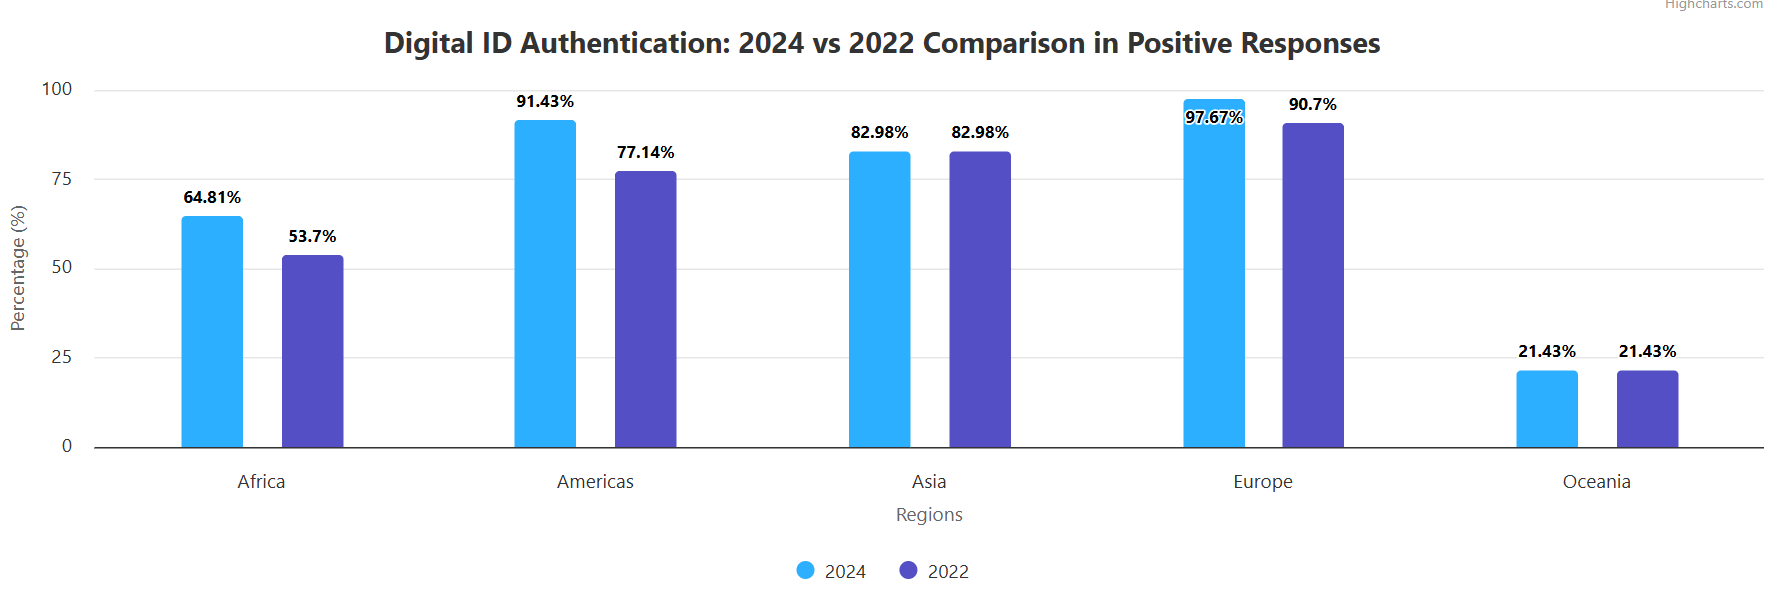
\includegraphics[width=1\linewidth]{figuras/digital_identity}
	\label{fig:national_identity}
	\footnotesize{Fonte: \cite{ONU_ICT_in_government_indicators}.}
\end{figure}

\begin{figure}[H]
	\centering
	\caption{Indicador de TIC de governo eletrônico: Existência de um portal de compras governamentais}
	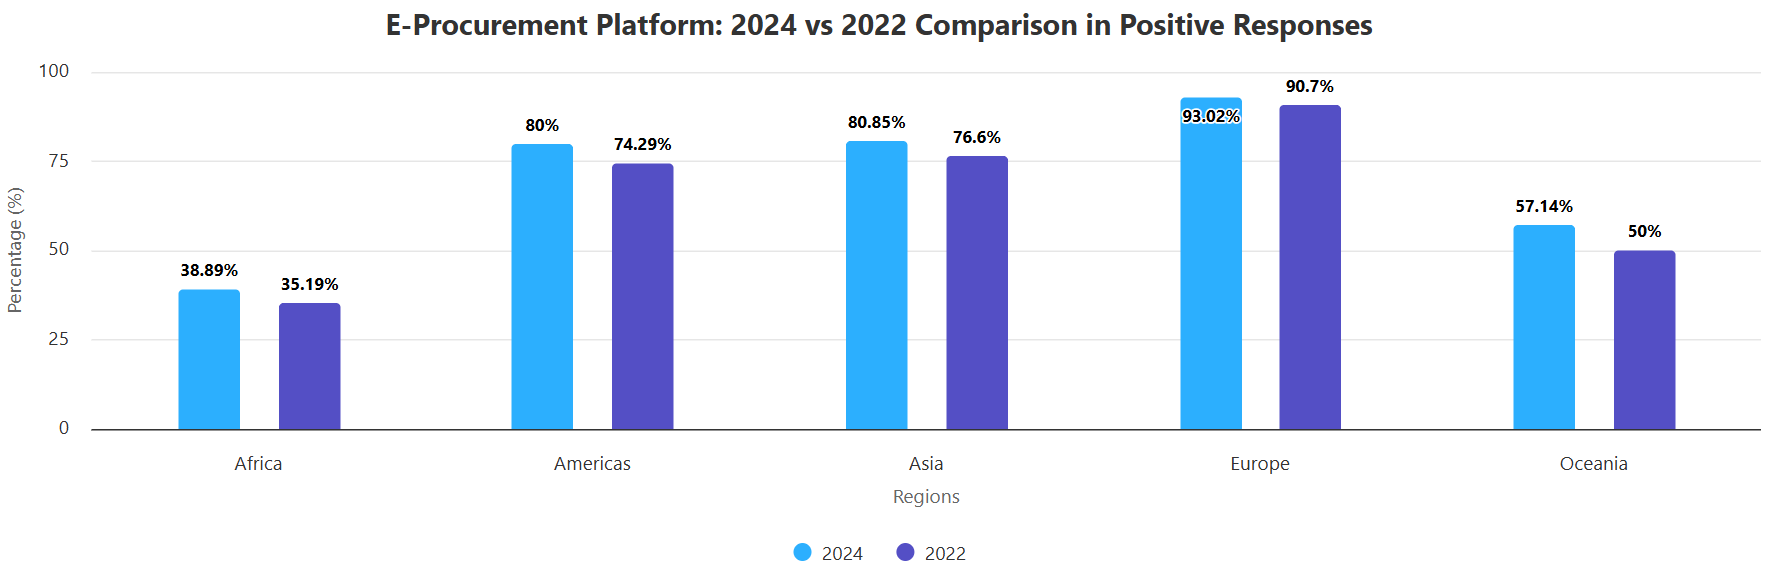
\includegraphics[width=1\linewidth]{figuras/procurement_portal}
	\label{fig:procurement_portal}
	\footnotesize{Fonte: \cite{ONU_ICT_in_government_indicators}.}
\end{figure}

Extraí-se das três figuras que a Europa foi o continente cujos mais respondem que têm seguido os indicadores, superando os 90\%. A Oceania foi o continente que menos implementou políticas de identidade digital para acesso a serviços digitais. África e Oceania tiveram um desempenho ruim na implementação de portais de compra governamentais. O continente americano apresentou bom desempenho nos três indicadores.

Como consequência da análise dos resultados presentes nas figuras \ref{fig:national_government_strategy}, \ref{fig:national_identity} e \ref{fig:procurement_portal}, buscou-se entender a seguinte situação registrada nos 2022 e 2024, anos em que os indicadores foram medidos: qual é a porcentagem de países que responderam nenhuma, uma, duas ou todas as perguntas. Elas usam sim ou não para confirmar a aplicação dos indicadores no país.

A resposta ao questionamento está presente na figura \ref{fig:ticegov_soma_respostas_positivas}.

\begin{figure}[H]
	\centering
	\caption{Respostas positivas aos indicadores de TIC de governo eletrônico de 2024}
	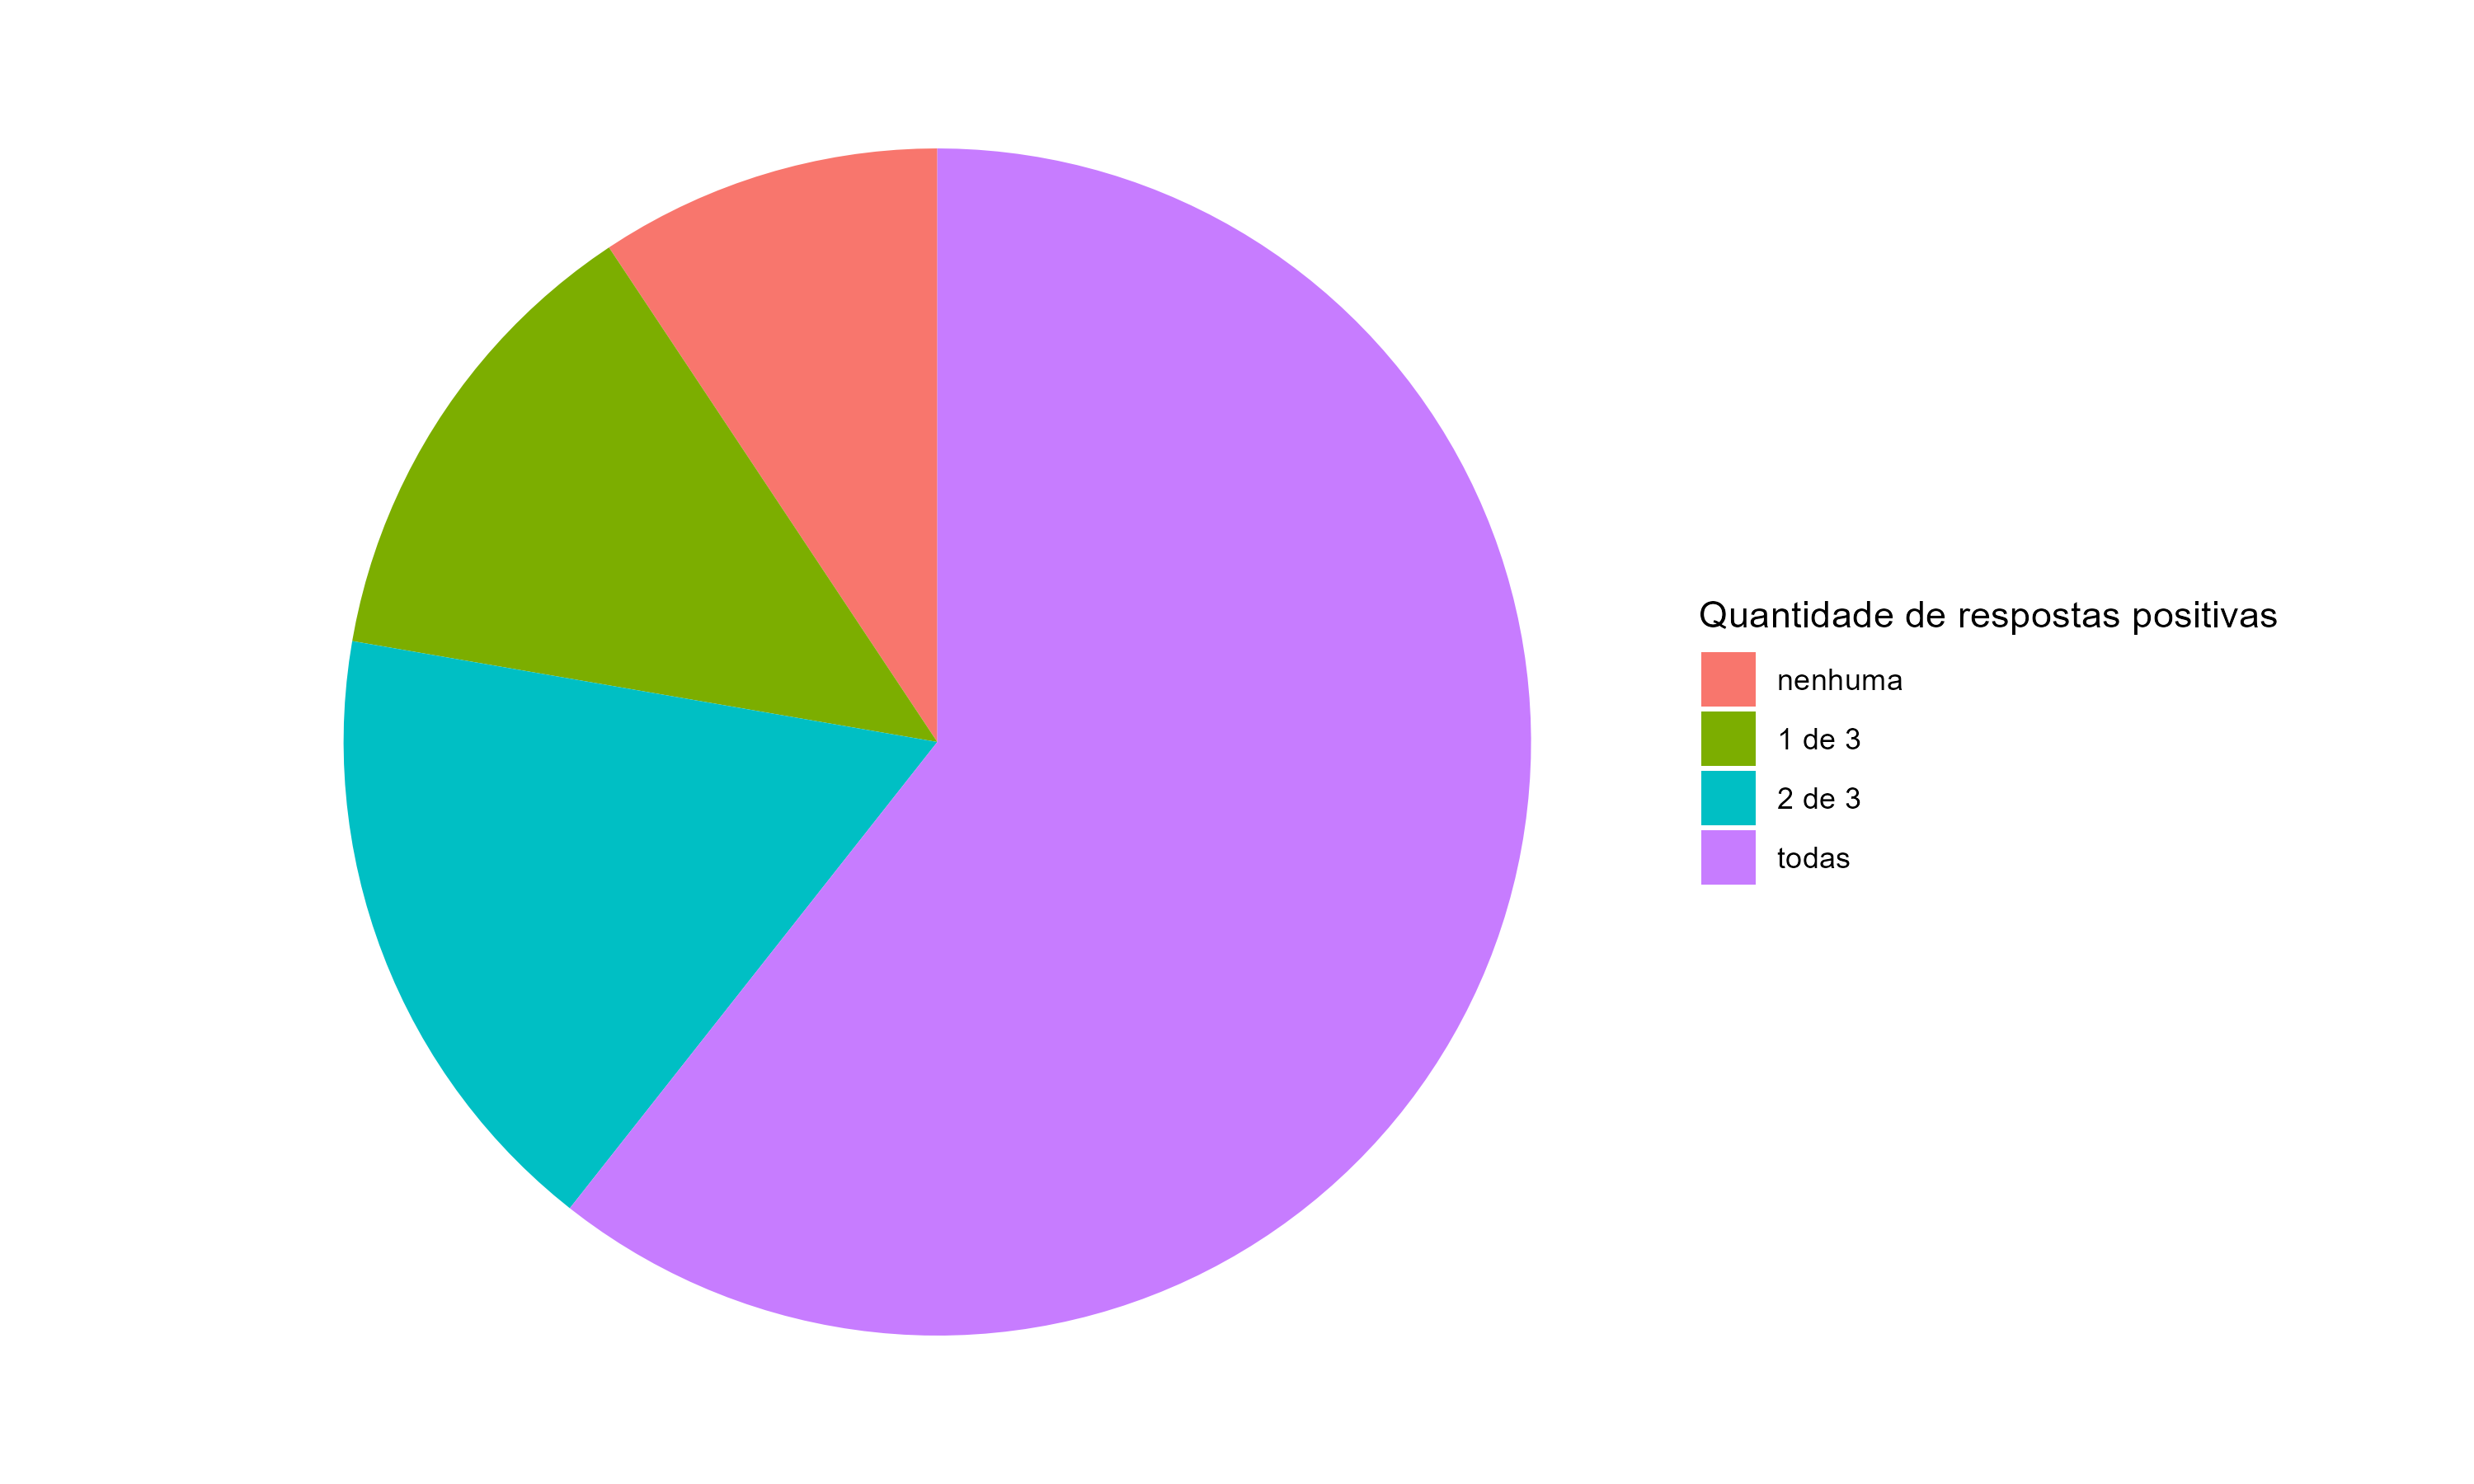
\includegraphics[width=1\linewidth]{figuras/ticegov_soma_respostas_positivas}
	\label{fig:ticegov_soma_respostas_positivas}
	\footnotesize{Fonte: \cite{ONU_ICT_in_government_indicators}.}
\end{figure}

Em 2024, mais da metade dos países respondeu positivamente às três perguntas. O Brasil faz parte desse grupo. Tal resultado indica que mais da metade dos países está investindo em TIC de governo eletrônico em seus territórios.

O resultado apresentado \textit{a priori} demonstra como o compromisso do Brasil com sua política pública de implementação, manutenção e a evolução do seu governo eletrônico.

No tocante ao indicador \textbf{existência de estratégia nacional de governo
eletrônico ou equivalente}, \cite{brasil_engd} cita que a Estratégia Nacional de Governo Digital (ENGD) está prevista na Lei do Governo Digital. A ENGD foi formalizada pelo Decreto nº 12.069, de 2024. E é complementada pela Portaria SGD/MGI nº 4.248, de 2024, que estabeleceu recomendações para o alcance dos objetivos da ENGD para o período de 2024 a 2027. Outras países também têm suas estratégias nacionais de governo eletrônico ou digital. São exemplos os Estados Unidos\footnote{cf. \url{https://www.state.gov/digital-government-strategy}} e Nigéria\footnote{cf. \url{https://fmcide.gov.ng/initiative/e-government-initiative/}}.

No tocante ao indicador \textbf{existência de identidade digital para acessar
ou outra forma de autenticação requerida para poder acessar serviços digitais}, ele foi alcançado no Brasil pela implementação da plataforma gov.br. 

Para \cite{mitkiewicz2024transformaccao}, a plataforma gov.br foi instituída em abril de 2019 pelo Decreto no 9.756 com o principal objetivo de integrar a oferta de serviços do governo federal para a população. 

\cite{mitkiewicz2024transformaccao} complementa que o decreto definiu forma, governança e prazos para a integração de portais e aplicativos dos órgãos públicos na internet ao novo portal e à loja única de aplicativos do governo federal, respectivamente. 

A norma estipulou o prazo de 31 de dezembro de 2020 para os órgãos e entidades da administração pública federal migrarem os conteúdos, de acordo com \cite{mitkiewicz2024transformaccao}.

Conforme \cite{mitkiewicz2024transformaccao} dispõe, o decreto 9.756 regulou ainda a organização do registro de domínios gov.br, obrigando, a partir de julho de 2019, a utilização do domínio raiz gov.br, seguido do complemento, para localizar os sítios de governo na internet. 

Para \cite{mitkiewicz2024transformaccao}, foi definido também o prazo de 31 de dezembro de 2020 para a desativação ou redirecionamento dos endereços eletrônicos existentes do governo federal. A norma definiu ainda o portal único gov.br como canal exclusivo para as ações de comunicação social e de utilidade pública do governo federal.

Para \cite{mitkiewicz2024transformaccao}, o Brasil possui uma trajetória de mais de duas décadas de planejamento e adoção de medidas estruturantes em diversas dimensões voltadas à implementação de uma visão de governo eletrônico/digital, abrangendo sete gestões presidenciais diferentes nesse período, sendo uma política pública de Estado.

O gov.br como canal de acesso único aos serviços públicos digitais é parte da iniciativa de Governo Digital apresentada no art. 3º, II da Lei 14.129, de 2021 - Lei do Governo Digital, conforme dispõe \cite{l14129}, \textit{ipsis litteris}: "Art. 3º  São princípios e diretrizes do Governo Digital e da eficiência pública: [...] II - a disponibilização em plataforma única do acesso às informações e aos serviços públicos, observadas as restrições legalmente previstas e sem prejuízo, quando indispensável, da prestação de caráter presencial;".

A Lei do Governo Digital também enquadra o gov.br dentro do conceito de \textbf{Governo como Plataforma} (art. 3º, XXIII), definido por \cite{l14129} como infraestrutura tecnológica que facilite o uso de dados de acesso público e promova a interação entre diversos agentes, de forma segura, eficiente e responsável, para estímulo à inovação, à exploração de atividade econômica e à prestação de serviços à população.

Como consequência, \cite{l14129} posiciona \textbf{Governo como Plataforma}, como: "XXIII - a implantação do governo como plataforma e a promoção do uso de dados, preferencialmente anonimizados, por pessoas físicas e jurídicas de diferentes setores da sociedade, resguardado o disposto nos arts. 7º e 11 da Lei nº 13.709, de 14 de agosto de 2018 (Lei Geral de Proteção de Dados Pessoais), com vistas, especialmente, à formulação de políticas públicas, de pesquisas científicas, de geração de negócios e de controle social;".

Outro aspecto fundamental do gov.br são as plataformas de governo digital, definidas por \cite{l14129} como ferramentas digitais e serviços comuns aos órgãos, normalmente ofertados de forma centralizada e compartilhada, necessários para a oferta digital de serviços e de políticas públicas. 

As plataformas de governo digital tem a seguinte estrutura, conforme \cite{l14129}, são instrumentos necessários para a oferta e a prestação digital dos serviços públicos de cada ente federativo, deverão ter pelo menos as seguintes funcionalidades: 

\begin{itemize}
    \item Ferramenta digital de solicitação de atendimento e de acompanhamento da entrega dos serviços públicos.
    \item Painel de monitoramento do desempenho dos serviços públicos.
\end{itemize}

O painel de monitoramento é regido pelo artigo 22 da Lei do Governo Digital, nos termos de \cite{l14129}, sendo o painel de monitoramento do desempenho dos serviços públicos de que trata o inciso II do caput do art. 20 deverá conter, no mínimo, as seguintes informações, para cada serviço público ofertado:

\begin{itemize}
    \item Quantidade de solicitações em andamento e concluídas anualmente.
    \item Tempo médio de atendimento.
    \item Grau de satisfação dos usuários.
\end{itemize}

Para confirmar a ideia expressa por \cite{mitkiewicz2024transformaccao} de que o Brasil tem políticas públicas de Estado de governo eletrônico e digital, \cite{painel_completo_monitoramento_govbr} apresenta os resultados (até 09/08/2025) do gov.br.

\begin{figure}[H]
    \centering
    \caption{Painel Detalhado do gov.br}
    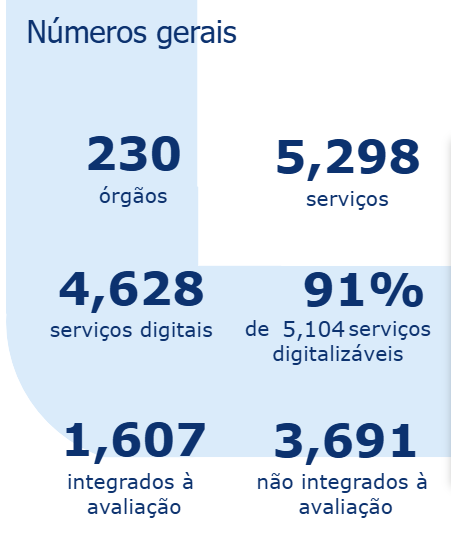
\includegraphics[width=0.5\linewidth]{figuras/painel_govbr.PNG}
    \label{fig:painel_govbr}
    \\ \footnotesize{Fonte: \cite{painel_completo_monitoramento_govbr}.}
\end{figure}

Com mais de 90\% dos serviços públicos digitalizados, comprova-se o motivo do EGDI do Brasil ser superior à média mundial. Outros países tem portais de acessso único similares ao gov.br. Tanto o Reino Unido\footnote{cf. \url{https://www.gov.uk/}}, quanto a Austrália\footnote{cf. \url{https://my.gov.au/}} tem seus portais único.

Finalmente, o último indicador de TIC de governo eletrônico - \textbf{existência de um portal de compras governamentais} foi implementado pela Lei nº 14.133, de 2021 - \textbf{Lei de Licitações e Contratos Administrativos}. A norma infraconstitucional, em concordância com \cite{l14133}, criou o Portal Nacional de Compras Públicas (PNCP), visando à divulgação centralizada e obrigatória dos atos exigidos pela lei e a realização facultativa das contratações pelos órgãos e entidades dos Poderes Executivo, Legislativo e Judiciário de todos os entes federativos.

\cite{l14133} expõe como condição indispensável para a eficácia do contrato e de seus aditamentos a divulgação no Portal Nacional de Compras Públicas, contados da data da assinatura, 20 dias úteis para licitações e 10 dias úteis para contratação direta.

De forma conclusiva, \cite{l14133} argumenta que os órgãos e entidades da Administração Pública deverão utilizar o sistema de registro cadastral unificado disponível no PNCP, para efeito de cadastro unificado de licitantes, na forma disposta em regulamento.
 
\subsection{Regressão polinomial do E-Government Development Index}

\section{GovTech Maturity Index}

\section{Digital Government Index}